% !BIB TS-program = biber
\RequirePackage[l2tabu,orthodox]{nag}
% TODO: decide if one-sided/two-sided
%\documentclass[headsepline,footsepline,footinclude=false,fontsize=11pt,paper=a4,listof=totoc,bibliography=totoc,BCOR=12mm,DIV=12]{scrbook} % two-sided
\documentclass[headsepline,footsepline,footinclude=false,oneside,fontsize=11pt,paper=a4,listof=totoc,bibliography=totoc]{scrbook} % one-sided
% TODO: change thesis information
\usepackage{graphicx}
\usepackage{tikz}

\usetikzlibrary{positioning}
\usetikzlibrary{calc,patterns}
\usetikzlibrary{shapes.geometric, arrows}
\tikzstyle{startstop} = [rectangle, rounded corners, minimum width=1cm, minimum height=1cm, text centered, draw=black]
\tikzstyle{process} = [rectangle, minimum width=1cm, minimum height=1cm, text centered, draw=black]
\tikzstyle{decision} = [diamond, minimum width=1cm, minimum height=1cm, text centered, draw=black]
\tikzstyle{arrow} = [thick,->,>=stealth]

\newcommand*{\getUniversity}{Technische Universität München}
\newcommand*{\getFaculty}{Informatics}
\newcommand*{\getDegree}{Informatics}
\newcommand*{\getSchool}{Computation, Information and Technology}
\newcommand*{\getTitle}{Tooling and Benchmarking of a Hardware-Agnostic Compilation Toolchain For Neutral-Atom Quantum Computers}
\newcommand*{\getTitleGer}{Tooling und Benchmarking einer hardwareunabhängigen Kompilierung Toolchain für Neutral-Atom Quantencomputer}
\newcommand*{\getAuthor}{Emil Khusainov}
\newcommand*{\getDoctype}{Bachelor's Thesis}
\newcommand*{\getSupervisor}{Prof. Dr. Christian Mendl}
\newcommand*{\getAdvisor}{M.Sc. Yanbin Chen}
\newcommand*{\getKeywords}{keyword;another keyword;one more}
\newcommand*{\getSubmissionDate}{04.07.2025}
\newcommand*{\getSubmissionLocation}{Munich}

% TODO: change citation style in settings
\PassOptionsToPackage{table,svgnames,dvipsnames}{xcolor}

\usepackage[a-2u]{pdfx} % generate PDF/A: archival compliant, self-contained pdf
\usepackage[utf8]{inputenc}
\usepackage[T1]{fontenc}
\usepackage[sc]{mathpazo}
\usepackage[ngerman,american]{babel}
\usepackage[autostyle]{csquotes}
\usepackage[%
  backend=biber,
  url=true,
  style=numeric,
  maxnames=4,
  minnames=3,
  maxbibnames=99,
  giveninits,
  uniquename=init]{biblatex} % TODO: adapt citation style
\usepackage{graphicx}
\usepackage{scrhack} % necessary for listings package
\usepackage{listings}
\usepackage{lstautogobble}
\usepackage{tikz}
\usepackage{pgfplots}
\usepackage{pgfplotstable}
\usepackage{booktabs}
\usepackage[final]{microtype}
\usepackage{caption}
\usepackage[printonlyused]{acronym}
\usepackage{ifthen}


\hypersetup{hidelinks} % removes colored boxes around references and links

% for fachschaft_print.pdf
\makeatletter
\if@twoside
	\typeout{TUM-Dev LaTeX-Thesis-Template: twoside}
\else
	\typeout{TUM-Dev LaTeX-Thesis-Template: oneside}
\fi
\makeatother

\addto\extrasamerican{
	\def\lstnumberautorefname{Line}
	\def\chapterautorefname{Chapter}
	\def\sectionautorefname{Section}
	\def\subsectionautorefname{Subsection}
	\def\subsubsectionautorefname{Subsubsection}
}

\addto\extrasngerman{
	\def\lstnumberautorefname{Zeile}
}

% Themes
\ifthenelse{\equal{\detokenize{dark}}{\jobname}}{%
  % Dark theme
  \newcommand{\bg}{black} % background
  \newcommand{\fg}{white} % foreground
  \usepackage[pagecolor=\bg]{pagecolor}
  \color{\fg}
}{%
  % Light theme
  \newcommand{\bg}{white} % background
  \newcommand{\fg}{black} % foreground
}

\bibliography{bibliography}

\setkomafont{disposition}{\normalfont\bfseries} % use serif font for headings
\linespread{1.05} % adjust line spread for mathpazo font

% Add table of contents to PDF bookmarks
\BeforeTOCHead[toc]{{\cleardoublepage\pdfbookmark[0]{\contentsname}{toc}}}

% Define TUM corporate design colors
% Taken from http://portal.mytum.de/corporatedesign/index_print/vorlagen/index_farben
\definecolor{TUMBlue}{HTML}{0065BD}
\definecolor{TUMSecondaryBlue}{HTML}{005293}
\definecolor{TUMSecondaryBlue2}{HTML}{003359}
\definecolor{TUMBlack}{HTML}{000000}
\definecolor{TUMWhite}{HTML}{FFFFFF}
\definecolor{TUMDarkGray}{HTML}{333333}
\definecolor{TUMGray}{HTML}{808080}
\definecolor{TUMLightGray}{HTML}{CCCCC6}
\definecolor{TUMAccentGray}{HTML}{DAD7CB}
\definecolor{TUMAccentOrange}{HTML}{E37222}
\definecolor{TUMAccentGreen}{HTML}{A2AD00}
\definecolor{TUMAccentLightBlue}{HTML}{98C6EA}
\definecolor{TUMAccentBlue}{HTML}{64A0C8}

% Settings for pgfplots
\pgfplotsset{compat=newest}
\pgfplotsset{
  % For available color names, see http://www.latextemplates.com/svgnames-colors
  cycle list={TUMBlue\\TUMAccentOrange\\TUMAccentGreen\\TUMSecondaryBlue2\\TUMDarkGray\\},
}

% Settings for lstlistings
\lstset{%
  basicstyle=\ttfamily,
  columns=fullflexible,
  autogobble,
  keywordstyle=\bfseries\color{TUMBlue},
  stringstyle=\color{TUMAccentGreen},
  captionpos=b
}


\begin{document}

% Set page numbering to avoid "destination with the same identifier has been already used" warning for cover page.
% (see https://en.wikibooks.org/wiki/LaTeX/Hyperlinks#Problems_with_Links_and_Pages).
\pagenumbering{alph}
\begin{titlepage}
  % HACK for two-sided documents: ignore binding correction for cover page.
  % Adapted from Markus Kohm's KOMA-Script titlepage=firstiscover handling.
  % See http://mirrors.ctan.org/macros/latex/contrib/koma-script/scrkernel-title.dtx,
  % \maketitle macro.
  \oddsidemargin=\evensidemargin\relax
  \textwidth=\dimexpr\paperwidth-2\evensidemargin-2in\relax
  \hsize=\textwidth\relax

  \centering

  \IfFileExists{logos/tum-\fg.pdf}{%
    \includegraphics[height=20mm]{logos/tum-\fg.pdf}
  }{%
    \vspace*{20mm}
  }

  \vspace{5mm}
  {\huge\MakeUppercase{School of \getSchool{} --- \getFaculty{}} \par}

  \vspace{5mm}
  {\large\MakeUppercase{\getUniversity{}} \par}

  \vspace{15mm}
  {\Large \getDoctype{} in \getDegree{} \par}

  \vspace{10mm}
  {\huge\bfseries \getTitle{} \par}

  \vspace{10mm}
  {\LARGE \getAuthor{}}

  \IfFileExists{logos/faculty-\fg.pdf}{%
    \vfill{}
    \includegraphics[height=20mm]{logos/faculty-\fg.pdf}
  }{}
\end{titlepage}


\frontmatter{}

\begin{titlepage}
  \centering

  \IfFileExists{logos/tum-\fg.pdf}{%
    \includegraphics[height=20mm]{logos/tum-\fg.pdf}
  }{%
    \vspace*{8mm}
  }

  \vspace{5mm}
  {\huge\MakeUppercase{School of \getSchool{} --- \getFaculty{}} \par}

  \vspace{5mm}
  {\large\MakeUppercase{\getUniversity{}} \par}

  \vspace{6mm}
  {\Large \getDoctype{} in \getDegree{} \par}

  \vspace{5mm}
  {\huge\bfseries \baselineskip=0.9\baselineskip \getTitle{} \par}

  \vspace{5mm}
  {\huge\bfseries \baselineskip=0.9\baselineskip  \foreignlanguage{ngerman}{\getTitleGer{}} \par}

  \vspace{6mm}
  \begin{tabular}{l l}
    Author:          & \getAuthor{}         \\
    Examiner:      & \getSupervisor{}     \\
    Supervisor:         & \getAdvisor{}        \\
    Submission Date: & \getSubmissionDate{} \\
  \end{tabular}

  \IfFileExists{logos/faculty-\fg.pdf}{%
    \vfill{}
    \includegraphics[height=20mm]{logos/faculty-\fg.pdf}
  }{}
\end{titlepage}

\thispagestyle{empty}
\vspace*{0.8\textheight}
\noindent
I confirm that this \MakeLowercase{\getDoctype{}} is my own work and I have documented all sources and material used.

\vspace{15mm}
\noindent
\getSubmissionLocation{}, \getSubmissionDate{} \hspace{\fill} \getAuthor{}

\cleardoublepage{}

\addcontentsline{toc}{chapter}{Acknowledgments}
\thispagestyle{empty}

\vspace*{20mm}

\begin{center}
    {\usekomafont{sectioning}\usekomafont{section} Acknowledgments}
\end{center}

\vspace{10mm}

%TODO: Acknowledgments

\cleardoublepage{}

\chapter{\abstractname}
\ac{NAQC} are new emerging architecture in the world of quantum computations. 
Its high fidelity, native multi-qubit gates and possibility to use in \ac{DPQA} features a lot of promises.
Moreover, \ac{DPQA} allows using physical shuttling of qubits during circuit execution instead or together with logical SWAP gates. 
All this opens up new compilation possibilities. 
Therefore, a new software tools that should take an advantage of additional capabilities of \ac{NAQC} are needed.
The goal of this work is to compare exiting tool chains for compilation, that took shuttling into account.
Moreover, the solutions will be balanced in places where they differ to compare the effectiveness of the algorithms they use and show inconsistencies in earlier benchmarks
\parencite{Tan_2025_Enola, Schmid_2024_NeutralAtomBasics}.

\microtypesetup{protrusion=false}
\tableofcontents{}
\microtypesetup{protrusion=true}

\mainmatter{}

% !TeX root = ../main.tex
% Add the above to each chapter to make compiling the PDF easier in some editors.

\chapter{Introduction}\label{chapter:introduction}

\section{Section}
Citation test~\parencite{latex}.

Acronyms must be added in \texttt{main.tex} and are referenced using macros. The first occurrence is automatically replaced with the long version of the acronym, while all subsequent usages use the abbreviation.

E.g. \texttt{\textbackslash ac\{TUM\}, \textbackslash ac\{TUM\}} $\Rightarrow$ \ac{TUM}, \ac{TUM}

For more details, see the documentation of the \texttt{acronym} package\footnote{\url{https://ctan.org/pkg/acronym}}.
\subsection{Subsection}

See~\autoref{tab:sample}, \autoref{fig:sample-drawing}, \autoref{fig:sample-plot}, \autoref{fig:sample-listing}.

\begin{table}[htpb]
  \caption[Example table]{An example for a simple table.}\label{tab:sample}
  \centering
  \begin{tabular}{l l l l}
    \toprule
      A & B & C & D \\
    \midrule
      1 & 2 & 1 & 2 \\
      2 & 3 & 2 & 3 \\
    \bottomrule
  \end{tabular}
\end{table}

\begin{figure}[htpb]
  \centering
  % This should probably go into a file in figures/
  \begin{tikzpicture}[node distance=3cm]
    \node (R0) {$R_1$};
    \node (R1) [right of=R0] {$R_2$};
    \node (R2) [below of=R1] {$R_4$};
    \node (R3) [below of=R0] {$R_3$};
    \node (R4) [right of=R1] {$R_5$};

    \path[every node]
      (R0) edge (R1)
      (R0) edge (R3)
      (R3) edge (R2)
      (R2) edge (R1)
      (R1) edge (R4);
  \end{tikzpicture}
  \caption[Example drawing]{An example for a simple drawing.}\label{fig:sample-drawing}
\end{figure}

\begin{figure}[htpb]
  \centering

  \pgfplotstableset{col sep=&, row sep=\\}
  % This should probably go into a file in data/
  \pgfplotstableread{
    a & b    \\
    1 & 1000 \\
    2 & 1500 \\
    3 & 1600 \\
  }\exampleA
  \pgfplotstableread{
    a & b    \\
    1 & 1200 \\
    2 & 800 \\
    3 & 1400 \\
  }\exampleB
  % This should probably go into a file in figures/
  \begin{tikzpicture}
    \begin{axis}[
        ymin=0,
        legend style={legend pos=south east},
        grid,
        thick,
        ylabel=Y,
        xlabel=X
      ]
      \addplot table[x=a, y=b]{\exampleA};
      \addlegendentry{Example A}
      \addplot table[x=a, y=b]{\exampleB};
      \addlegendentry{Example B}
    \end{axis}
  \end{tikzpicture}
  \caption[Example plot]{An example for a simple plot.}\label{fig:sample-plot}
\end{figure}

\begin{figure}[htpb]
  \centering
  \begin{tabular}{c}
  \begin{lstlisting}[language=SQL]
    SELECT * FROM tbl WHERE tbl.str = "str"
  \end{lstlisting}
  \end{tabular}
  \caption[Example listing]{An example for a source code listing.}\label{fig:sample-listing}
\end{figure}

% !TeX root = ../main.tex
% Add the above to each chapter to make compiling the PDF easier in some editors.

\chapter{Related Work}\label{chapter:relatedwork}
In this work different compilation toolchains for neutral atom architecture are considered \parencite{huang2025dasatomdivideandshuttleatomapproach,Tan_2025_Enola, schmid2023hybridcircuitmappingleveraging}.
The global goal is to determine the impact of qubit shuttling onto overall circuit fidelity and amount of gates.
Moreover, during this work will be determined drastic mismatches in benchmarks of considered toolchains. 
And a step in direction to possible fair comparison is done.

As a related work consider \parencite{gao2025optimalcompilationstrategiesqft}.
In it author tries to show possible mismatches in results of compilation because of minimal input parameters deviations, 
often substantial and difficult to rationalize discrepancies. 
Therefore, raising an important issue of fair evaluation, 
which is essential for understanding which approaches perform better or worse.

\section{Approach}
The idea of this work is to bench different tools for neutral atom compilation to understand what approaches are better 
and what considered hardware constraints raise significant impact on overall compilation quality.
Similarly, it is important to consider the other side of the problem shown by \parencite{gao2025optimalcompilationstrategiesqft}.
This aspect involves not only comparing discrepancies resulting by differences in input values, 
but also to determine the reasons why a minority of these inputs made the compilation process ill-conditioned.
% !TeX root = ../main.tex
% Add the above to each chapter to make compiling the PDF easier in some editors.

\chapter{Background}\label{chapter:background}
\section{Quantum Basics}
\subsection{Idea of Quantum Computation}
For more than 50 years of using classical paradigms of computations it has been recognized, 
that parallel to classical ones exists also a quantum version of them \parencite{Barenco_1995}.
Which offers clearly different and perhaps much more powerful features than classical computational theory
\parencite{Markov_2014,article}.

\subsection{Quantum State and its Representation}
The following section is primarily based on \parencite{nielsen00} supplemented by \parencite{article,Markov_2014}. 

Quantum mechanics uses operations with states in a complex Hilbert space to perform computations.
This quantum state serves as an analog of an ordinary bit in the quantum world. 
In the following considered only one-qubit system for simplicity w.l.o.g. in so-called computational basis.
Moreover, this state possesses not only basis states \(|0\rangle\) and \(|1\rangle\),
but also an infinite amount of combinations of this eigenstates, this is called a quantum superposition. 
To represent it two complex numbers \(\alpha\) and \(\beta\) are used.
For one-qubit system we define a quantum state as follows:
\[
|\psi\rangle = \alpha|0\rangle + \beta|1\rangle
\]
The coefficients must satisfy the following normalization condition:
\[
|\alpha|^2 + |\beta|^2 = 1
\]
To transfer quantum information into classical bits a measurement operation is performed.
Measurement will always collapse a wave function into one of corresponding to result the basis states. 
The probability of outcome is calculated with Born's rule as follows:
\[
P(0) = |\alpha|^2, \quad P(1) = |\beta|^2
\]
For visualization, the state can be represented geometrically as vector in Bloch Sphere, 
where angles \(\theta\) and \(\phi\) will uniquely determine the position of the vector. 
\[
|\psi\rangle = \cos\frac{\theta}{2}|0\rangle + e^{i\phi}\sin\frac{\theta}{2}|1\rangle
\]

%\[|\psi\rangle \otimes |0\rangle \rightarrow |\psi\rangle \otimes |\psi\rangle \]

%\[|\Phi^+\rangle = \frac{|00\rangle + |11\rangle}{\sqrt{2}}\]

%\subsection{Quantum Gates}

% !TeX root = ../main.tex
% Add the above to each chapter to make compiling the PDF easier in some editors.

\chapter{Neutral Atom Architecture}\label{chapter:neutralatom}
There are already a considerable amount of approaches for building a \ac{QC}.
All of them are based on different physical systems that manage the creation, connection and manipulation of qubits \parencite{Wintersperger_2023}.
Several of the promising approaches are:
%\section{DiVichenzo Criteria?}
\section{Prevalent Architectures}
\subsection{Superconducting Qubits}
The main insights into this technology have been collected by \parencite{Huang_2020}. 
This architecture uses superconducting resonant circuits, which apply microwave signals to control and read qubits. 

The strong sites are its very fast single- and two-qubit gates,
electronics that cover current needs have been around for a long time and have been well studied 
e.g. commercial microwave devices can be used in experiments,
an increase of qubit amount in moderate effort is possible, 
different types of qubits \ref{fig:superconducting} and parameters with easy coupling nature of qubits allow high designability.

The week sides are necessity in close to absolute zero temperature to operate, strongly limited coherence times, 
crosstalk between qubits requires careful design, complex error correction mechanisms,
a qubit is not true two-level system, thus undesired transitions must be avoided during processing.
\begin{figure}[htbp]
  \centering
    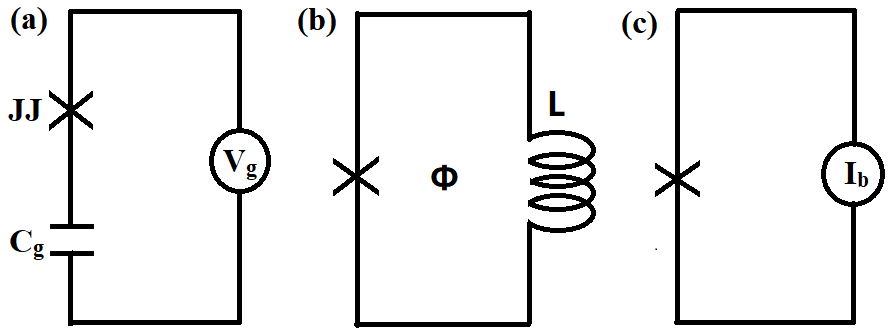
\includegraphics[width=0.8\textwidth]{figures/Superconducting.png}
    \caption{Three types of superconducting qubits circuit diagrams \parencite{Huang_2020}}
    \label{fig:superconducting}
    %referring by label \ref{fig:your-label}.
\end{figure}

\subsection{Photons}
Key concepts of this technology are drawn from the work \parencite{romero2024photonicquantumcomputing}.
Uses photons as qubits and raise several points; computations are done via beam splitters, phase shifters, and detectors.

To advantages could be assigned operations with interference and entanglement by room temperatures,
low decoherence due to weak interaction with environment,
could bring a significant potential in the networks of quantum computers in the future.

Meanwhile, disadvantages include necessity in high-quality hardware to save and detect states,
complex error correction techniques and hard scaling.

\subsection{Topological}
The main insights into this technology have been collected by \parencite{Lahtinen_2017, Zhang_2024}.
Encodes information non-locally using non-abelian anions such as Majorana zero modes in topological superconductors 
or exotic materials. 
Logical gates are implemented via braiding operations which are inherently error-resistant.


Advantages are built-in topological protection which enhances resilience to local noise, 
potentially reducing error correction complexity.

Disadvantages are hard experimental realization of stable non-abelian anions,
several operations are still theoretical or nascent.
\subsection{Ion Traps}
Key concepts of this technology are drawn from the work \parencite{Bruzewicz_2019}.
Uses positive ions such as Yb or Ca  placed in electromagnetic traps. 
Qubit states are encoded in stable electronic levels.

The strong sites are high coherence time, that can be exceptionally long also without applying of decoupling techniques,
high fidelity of one-qubit and two-qubit gates, straightforward state preparation and readout.

The weak side is non-trivial scaling over fifty ions due to heating and crowding processes.
\section{Neutral Atom}
The main considered physical architecture of this paper is \ac{NAQC}. 
This type of computer uses laser cooling and trapping techniques for neutral atoms and
optical or microwave pulses to manipulate quantum states.  
It offers long coherence times, scaling in 1D, 2D or even 3D,
and fair connectivities by long-range interactions between atoms in Rydberg state \parencite{Wintersperger_2023}.
\subsection{Physical Hardware Implementation}
Consider \ref{fig:ColdAtomArchitecture} to have a schematic overview.
Neutral atoms such as Rubidium, Cesium or Strontium are positioned inside an ultra-high vacuum cell 
in a specific geometric arrangement, typically achieved by optical tweezers. 
To work with it, it needs to be cooled to low temperatures.
The process of cooling is multistaged that especially involves Doppler cooling using a laser.
To place cooled atoms on fixed locations and keep them a trap laser controlled by \ac{SLM} is employed.
With help of \ac{SLM} laser could be focused onto very small configurable points, this effect called optical tweezers.
\ac{SLM} could arrange atoms in 1D, 2D,or even in 3D configuration.
To move atoms there are another mobile traps controlled by \ac{AOD}.
\ac{AOD} implements the comparable to \ac{SLM} function, but for mobile optical tweezers.
Then all electronics should be precisely calibrated to control process run \parencite{Schmid_2024_NeutralAtomBasics, Wintersperger_2023}.

To perform actually computations laser and microwaves are employed, 
depends on executed gate used so-called Raman or Rydberg pulses, 
which could work locally or globally on arrangement of neutral atoms. 
\parencite{Schmid_2024_NeutralAtomBasics, Wintersperger_2023}
\begin{figure}[htbp]
  \centering
    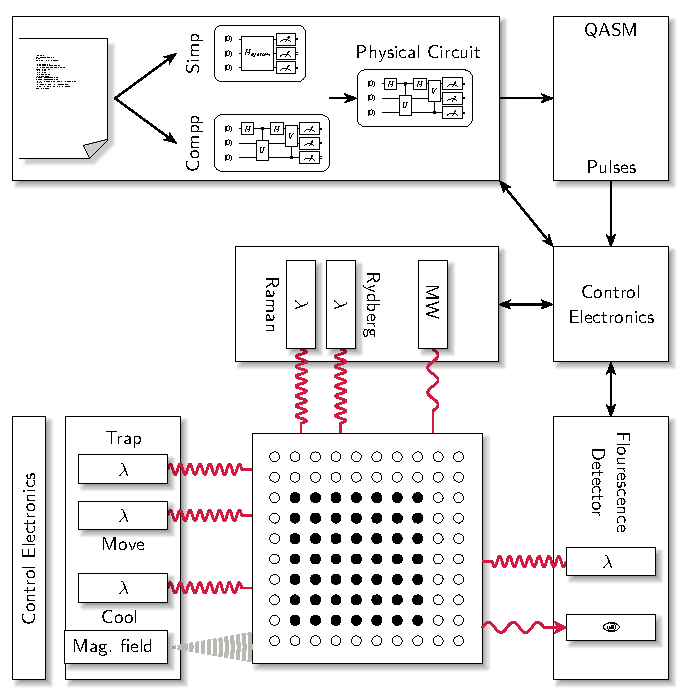
\includegraphics[width=0.8\textwidth]{figures/ColdAtomArchitecture.pdf}
    \caption{Schematic component overview of a cold atom quantum computer \parencite{Wintersperger_2023}}
    \label{fig:ColdAtomArchitecture}
\end{figure}

\subsection{Processing}
According to \parencite{Wintersperger_2023, Philipp_Wondra_TUM_Thesis_for_Informatics.pdf}.
To use neutral atoms for performing quantum computations
encoding of qubit computation basis state needs to be determined.
These encoding should have a long coherence time and weak interaction with environment.
For Rubidium atom it is based on the spin of the furthest electron. 
Meanwhile, a Strontium implementation a nuclear spin of atom is used.

For implementing a one-qubit rotations operators two laser induced known as Raman transition are used.
Target atom exposure to multiple photons and after that emits some another amount of energy,
what led to change of it state, by combining the duration, power and frequency of laser  
different direction and angles of rotation could be achieved.

For implementing a two-qubit gates a so-called Rydberg state is used. 
In this state an outermost electron has a very huge influence on other atoms' electrons in arrangement.
Thus, other atom can not go in Rydberg state. This effect widely known as Rydberg blockade.
An effective impact of this effect is an implementation of a Controlled-Z gate.

Moreover, this effect enables the implementation of multiple-controlled Z-Gate directly on hardware,
since Rydberg blockade influences not only neighboring qubits but extends as a distance-dependent interaction.
The strength of blockade obeys the proportion for small distances \(\frac{1}{|r|^3}\) and \(\frac{1}{|r|^6}\) for long.
Depending on a coefficient that accepted for blocking and interacting, 
different multiple-controlled Z-Gate are implemented.

In addition, Rydberg blockade effect is used for long-range interactions between qubits within the acceptable distance, 
it is with \ac{NAQC} possible to execute a two-qubit gate 
and do not require specifically to place the atoms directly next to each other.

Nevertheless, if an interaction radius is small for gate execution,
logical SWAP gates are considered to logically move qubit to the target qubit.
But \ac{DPQA} could be based on neutral atoms. 
Hence, it makes possible to use physical moving of qubit in lattice, by moving it from \ac{SLM} to \ac{AOD} and back.
This process is known as qubit shuttling.

For visualization of the described features consider \ref{fig:NeutralAtomFeatures}.

\begin{figure}[htbp]
  \centering
    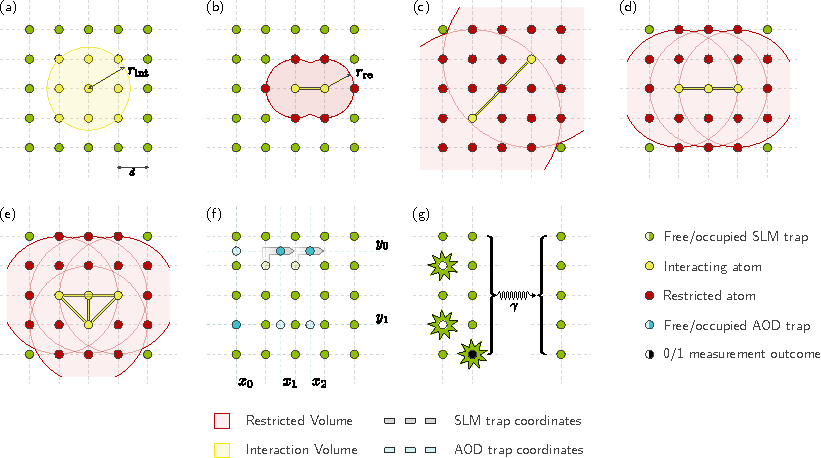
\includegraphics[width=0.8\textwidth]{figures/NeutralAtomFeatures.pdf}
    \caption[Capabilities of the NAQC platform.]{\textbf{Capabilities of the NAQC platform.} In this setup, atoms are arranged on a regular grid of \ac{SLM} traps, with a fixed distance denoted as $d$.
  \textbf{(a)} Rydberg blockade interaction: interacting gates can be performed to all qubits within this range.
  \textbf{(b)} Two-qubit gate: A gate can be applied between neighboring qubits but restricts the simultaneous execution of other entangling gates on nearby atoms.
   \textbf{(c)} Long-Range interactions: For gates with larger interaction radii, the restriction zones also expand, resulting in more restricted atoms.
  \textbf{(d)} CCZ gate with a line arrangement of the qubits. 
  According to \cite{Levine_2019} it is sufficient if the central atom interacts with both the outer qubits.
  \textbf{(e)} CCCZ gate 
  \textbf{(f)} Shuttling operation: \ac{AOD} (blue) enable the movement of atoms within the same column or row.
  \textbf{(g)} Additional NA capabilities, useful for future fault-tolerant computations. Not relevant for this work
   \parencite{Schmid_2024_NeutralAtomBasics}.
}\label{fig:NeutralAtomFeatures}
\end{figure}

% !TeX root = ../main.tex
% Add the above to each chapter to make compiling the PDF easier in some editors.

\chapter{Compilation in \ac{NAQC}}\label{chapter:compilation}
Compilation is a process of translating a high-level, 
abstract description of a quantum algorithm into a low-level representation of operations suitable for hardware execution.
To achieve it, this problem is divided into multiple subproblems, 
employing different layers of software each for specific subproblems, well-known as compilation toolchain.
Moreover, compilation should be familiar with computational capabilities of target hardware.
As described in \ref{chapter:neutralatom} each compilation step for \ac{NAQC} should consider further hardware constraints.

Described by \parencite{Tan_2025_Enola,Schmid_2024_NeutralAtomBasics}; 
For example, that together with SWAP or instead of SWAP-based losing of connectivity problem
there is also possible to shuttle qubit physical, 
compiler should be able to calculate which way will be the most efficient in terms of speed, fidelity, calculation time in the specific situation.

Hence, compiler should consider different execution times of gates, their fidelities, 
and also an available set of gates on current machine.

Moreover, compiler should consider idle time of qubits and calculate corresponding impact from coherence time.
Thus, it should now which operations could be executed parallel and what properties do \ac{AOD} and \ac{SLM} have.

Nevertheless, compiler should consider possible different grid architectures as described in \ref{chapter:neutralatom} 
to take advantage from different lattice realizations. 
Consequently, as described in \ref{chapter:neutralatom} interaction is not restricted only for interacting qubits but decays with distance, 
following an inverse cubic law.  

Also, compiler should consider different interaction radius and Rydberg blockade radius, 
and schedule next step according to constraints that go from previous steps and architecture, 
to improve overall quality of compilation.

\section{Compilation Steps}
Consider \ref{fig:compilation_steps}.
\begin{figure}[htbp]
  \centering
    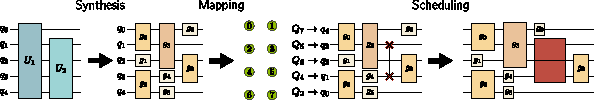
\includegraphics[width=0.8\textwidth]{figures/compilation_steps.pdf}
    \caption[Illustration of the three steps for platform-dependent compilation]{\textbf{Illustration of the three steps for platform-dependent compilation.} In the \textbf{synthesis} step, general operations and unitaries are decomposed into the native gate set $\Sigma_{\mathrm{native}}$.
  During the \textbf{mapping} step, the circuit qubits $q_{i}$ are assigned to physical hardware qubits $Q_{i}$, and necessary SWAP or MOVE operations are introduced to satisfy connectivity constraints.
  Finally, in the \textbf{scheduling} step, gate times and restrictions on parallelism are considered.
  In practice, these steps are often performed simultaneously as a single step rather than sequentially. \parencite{Schmid_2024_NeutralAtomBasics}}
    \label{fig:compilation_steps}
\end{figure}

\section{Considered Toolchains}
In this work three Compiling Toolchains for \ac{NAQC} are considered, 
since they take a QASM circuit as import and are open-source python projects \parencite{Tan_2025_Enola,schmid2023hybridcircuitmappingleveraging,huang2025dasatomdivideandshuttleatomapproach}.
This chapter will cover algorithms that are used by these three, 
describe a workflow, what tools each toolchain uses, and what is considered by compilation.
Nevertheless, the result of benchmarking will be evaluated in the next chapter.

\subsection{HybridMapper MQT}
HybridMapper, a tool from \ac{MQT}, stands out from the previous works, 
because it uses a hybrid compilation approach to map a circuit 
and considers together SWAP gates and shuttling to explore the potential advantage of leveraging gate-based SWAP insertions 
and shuttling-based atom rearrangements \parencite{schmid2023hybridcircuitmappingleveraging}.
When other works individually only considered it separately \parencite{Tan_2025_Enola,huang2025dasatomdivideandshuttleatomapproach,10082942}.
In particular, this is only a mapping and scheduling stage of computation, without synthese and optimization steps.
The process takes a QASM circuit as input and uses only gates that defined with architecture along with their times, and fidelities.
\ac{HybridMapper} does not optimize circuit or change something in there, it finds places where interacting conditions are violated 
and solves it with logical or physical move according to internal cost function \parencite{schmid2023hybridcircuitmappingleveraging}. 
In advance, skipping synthese step gives advantages, 
since other considered toolsets always try to transpile input circuit into Pauli Gates and CZ gate, without consideration of possible multi-qubit CZ gates \parencite{schmid2023hybridcircuitmappingleveraging}.

The main idea of algorithm is to use two-capability-specific heuristic cost functions, 
which specially made for fast evaluation 
and consider additional architecture information 
such as number of \ac{AOD} or \ac{SLM} traps, distance between them, interaction radius 
to improve parallelism by using commutation rules and look-ahead functionality \parencite{schmid2023hybridcircuitmappingleveraging}.
Consider for accuracy \ref{fig:overview_HybridMapper}.

\begin{figure}[htbp]
  \centering
    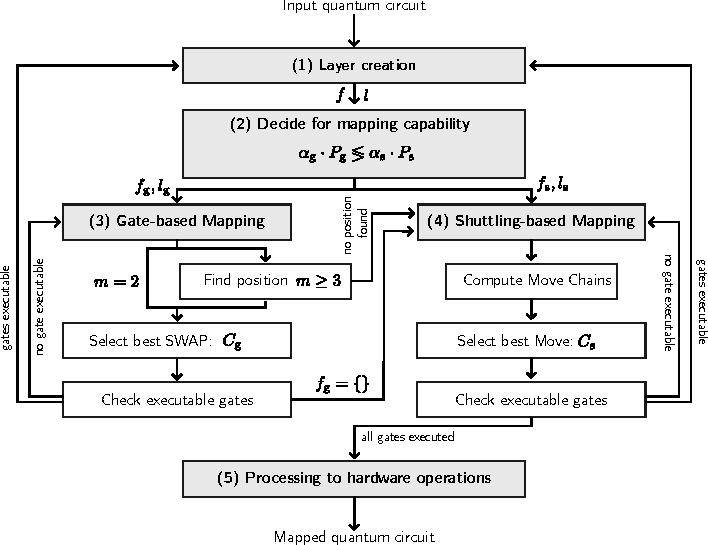
\includegraphics[width=0.8\textwidth]{figures/overviewHybridMapper.pdf}
    \caption{Resulting hybrid mapping process \parencite{schmid2023hybridcircuitmappingleveraging}}
    \label{fig:overview_HybridMapper}
\end{figure}
\subsection{Enola}
Enola a Tool from \ac{UCLA-VAST} based on OLSQ-DPQA uses different approach \parencite{Tan_2025_Enola,Tan_2024}.
It divides mapping and scheduling steps of compilation into scheduling, placement and routing steps to achieve excellent fidelity.

Scheduling step is implemented thorough Edge Coloring problem of commutation group (a group consisting of commutable two-qubit
gates that can be executed in any order) graph, 
where vertices are qubits and edges are two-qubit gates. 
This problem then is solved using Misra-Gries algorithm.
For more generic circuits Enola can use the dependency DAG (directed acyclic graph) for the two-qubit
gates in a generic circuit. In this case, the scheduling problem is
straightforward: the optimal number of stages is the critical path
in the DAG and ASAP (as soon as possible) scheduling can achieve
optimality \parencite{Tan_2025_Enola}. 
Visualization \ref{fig:scheduling_Enola}
\begin{figure}[htbp]
  \centering
    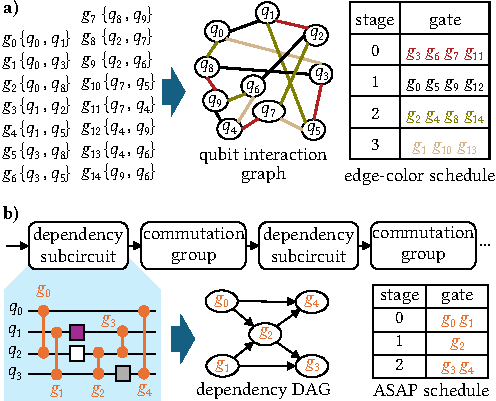
\includegraphics[width=0.8\textwidth]{figures/scheduling_Enola.pdf}
    \caption [Scheduling in Enola]{ Scheduling in Enola. 
    \textbf{(a)} Scheduling a commutation group of two-qubit gates with edge coloring. 
    \textbf{(b)} Generic circuits can be divided to dependency subcircuits and commutation groups. 
    Dependency subcircuits are scheduled ASAP \parencite{Tan_2025_Enola}.}
    \label{fig:scheduling_Enola}
\end{figure}

Placement step is implemented through fast simulated annealing algorithm, 
qubits are mapped to interaction sited and the two-qubit
gates at each Rydberg stage are like 2-pin nets in conventional
circuit placement. Hence, the goal is to minimize total "wire-length".
Fast simulated annealing has three-stages to explore possible states.
At the first stage random search to explore a large solution space is used, the so-called temperature is high, 
thus a probability of bad solution is high.
Then, the second stage is a pseudo-greedy local search. 
The last stage is a hill-climbing search where
the temperature increases again to escape from local minima \parencite{Tan_2025_Enola}. 
Visualization \ref{fig:placement_Enola}.
\begin{figure}[htbp]
  \centering
    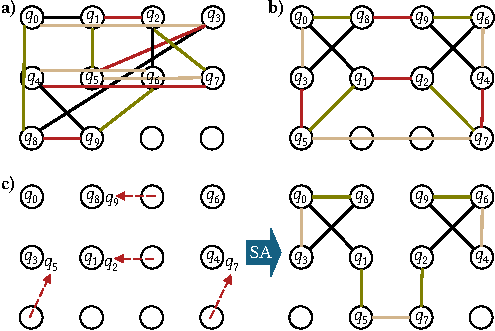
\includegraphics[width=0.8\textwidth]{figures/placement_Enola.pdf}
    \caption[Placement in Enola]{ Placement in Enola. 
    \textbf{(a)} Trivial placement from left to right, from top to bottom. 
    \textbf{(b)} Placement with gate distance optimized by simulated annealing. 
    \textbf{(c)} Dynamic placement: after a Rydberg stage (red) is executed (left), run simulated
    annealing on moved qubits for a new placement (right). \parencite{Tan_2025_Enola}}
    \label{fig:placement_Enola}
\end{figure}

Routing step is used to parallelize the \ac{AOD} movements, 
and not to violate fundamental rules of \ac{AOD} such as \textit{the order of its columns cannot change, nor can
the order of rows}.
Then the independent set of vertices is made of possible moves. 
This set will be solved then with maximum independent set solver \parencite{Tan_2025_Enola}.
Visualization \ref{fig:routing_Enola}.
\begin{figure}[htbp]
  \centering
    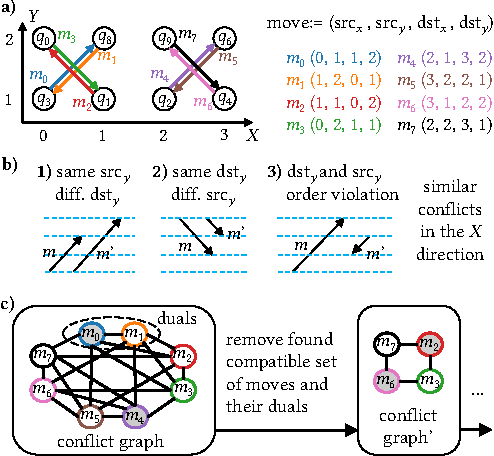
\includegraphics[width=0.8\textwidth]{figures/routing_Enola.pdf}
    \caption[Routing in Enola]{Routing in Enola. 
    \textbf{(a)} Definition of a move as a 4-tuple. 
    \textbf{(b)} Conflicts between two moves. 
    \textbf{(c)} Compatible moves are independent sets (IS) in the conflict graph (filled vertices).
    After finding an IS, delete the moves and their duals from
    the graph. The process continues until no moves are left \parencite{Tan_2025_Enola}.}
    \label{fig:routing_Enola}
\end{figure}

Additionally, Enola transpiles input circuit into fixed gate set from Pauli Gates and CZ, 
without consideration of a big advantage of \ac{NAQC} that allows to implement different gates.
Nevertheless, it considers interaction radius, Rydberg blockade radius, durations and fidelities of gates,
physical placement of \ac{SLM} and \ac{AOD} traps. 
An important note is that Enola does not consider number of \ac{AOD}, 
but make an independent set of gates so-called stages where each pair of gates could be executed without affecting other qubits in corresponding stage \parencite{Tan_2025_Enola}.

\subsection{DasAtom}
DasAtom was made as an improvement of Enola and Tetris 
and used the weakest aspects of each to strengthen them and made itself.
Enola leverages atom shuttling to adapt qubit mappings dynamically,
but cannot take advantage of long-range interactions
and Tetris' main idea is to leverage the long-range interactions of \ac{NAQC} 
to achieve denser qubit connectivity \parencite{10082942,Tan_2025_Enola, huang2025dasatomdivideandshuttleatomapproach}.

The main idea of DasAtom is a slightly changed \ac{DAC} approach to divide circuit into subcircuits.
It was inspired from different DAC adaptations from \parencite{siraichi:hal-02316820, 10.1145/3508352.3549394, huang2024qubitmappingadaptivedivideandconquer}
Then it assigns an optimal qubit mapping for each subcircuit, and then shuttles
atoms to smoothly transition between mappings. This approach should improve overall fidelity and efficiency \parencite{huang2025dasatomdivideandshuttleatomapproach}.
Consider \ref{fig:DasAtomFlowChart}

\begin{figure}
\centering
\scalebox{0.78}{
\begin{tikzpicture}[node distance=1.5cm]

% Nodes
\node (start) [startstop] {Input: CZ circuit $C$, $d$, $R_{\mathrm{int}}$, $R_{\mathrm{restr}}$};
\node (partition1) [process, below of=start] {Divide $C$ into CZ layers $L_1,...L_m$};
\node (partition2) [process, below of=partition1] {Divide $C$ into $C_1, ..., C_k$ and find an embedding $f_i$ for each $C_i$};
%\node (init) [process, below of=partition2] {Let $i = 1$};
\node (execute) [process, below of=partition2] {Start with $i=1$ and execute $C_i$ with $f_i$};
\node (decision) [decision, below of=execute, yshift=-0.5cm] {$i = k?$};
\node (route) [process, below of=decision, yshift=-0.5cm] {Route $f_i$ to $f_{i+1}$};
\node (increment) [process, left of=route, xshift=-2.5cm] {$i = i + 1$};
\node (end) [startstop, right of=decision, xshift=1.5cm] {End};
% Arrows
\draw [arrow] (start) -- (partition1);
\draw [arrow] (partition1) -- (partition2);
\draw [arrow] (partition2) -- (execute);
\draw [arrow] (execute) -- (decision);
\draw [arrow] (decision) -- node[anchor=east] {no} (route);
\draw [arrow] (route) -- (increment);
\draw [arrow] (increment) |- (execute.west);
\draw [arrow] (decision) -- node[anchor=south] {yes} (end);

\end{tikzpicture}}
\caption{The flowchart of DasAtom \parencite{huang2025dasatomdivideandshuttleatomapproach}.}
\label{fig:DasAtomFlowChart}
\end{figure}

DasAtom states about 415.8 times higher fidelity comparing to Enola in \ac{QFT}30. 
This statement seems to be only partially correct.
\parencite{huang2025dasatomdivideandshuttleatomapproach}
% !TeX root = ../main.tex
% Add the above to each chapter to make compiling the PDF easier in some editors.

\chapter{Evaluation of Framework}\label{chapter:evaluation}
For benchmarking of discussed in \ref{chapter:compilation} compilation tool chains a python project was introduced \parencite{Emil_Khusainov_Bachelor_GIT}.
The initial objective was to compare these three tool chains with architectures as similar as possible.
\section{Implementation and testing nuances}
For those purposes the following program structure were made \ref{fig:overview}.
As Test Cases several \ac{QFT} circuits are used.
\begin{figure}[htbp]
  \centering
    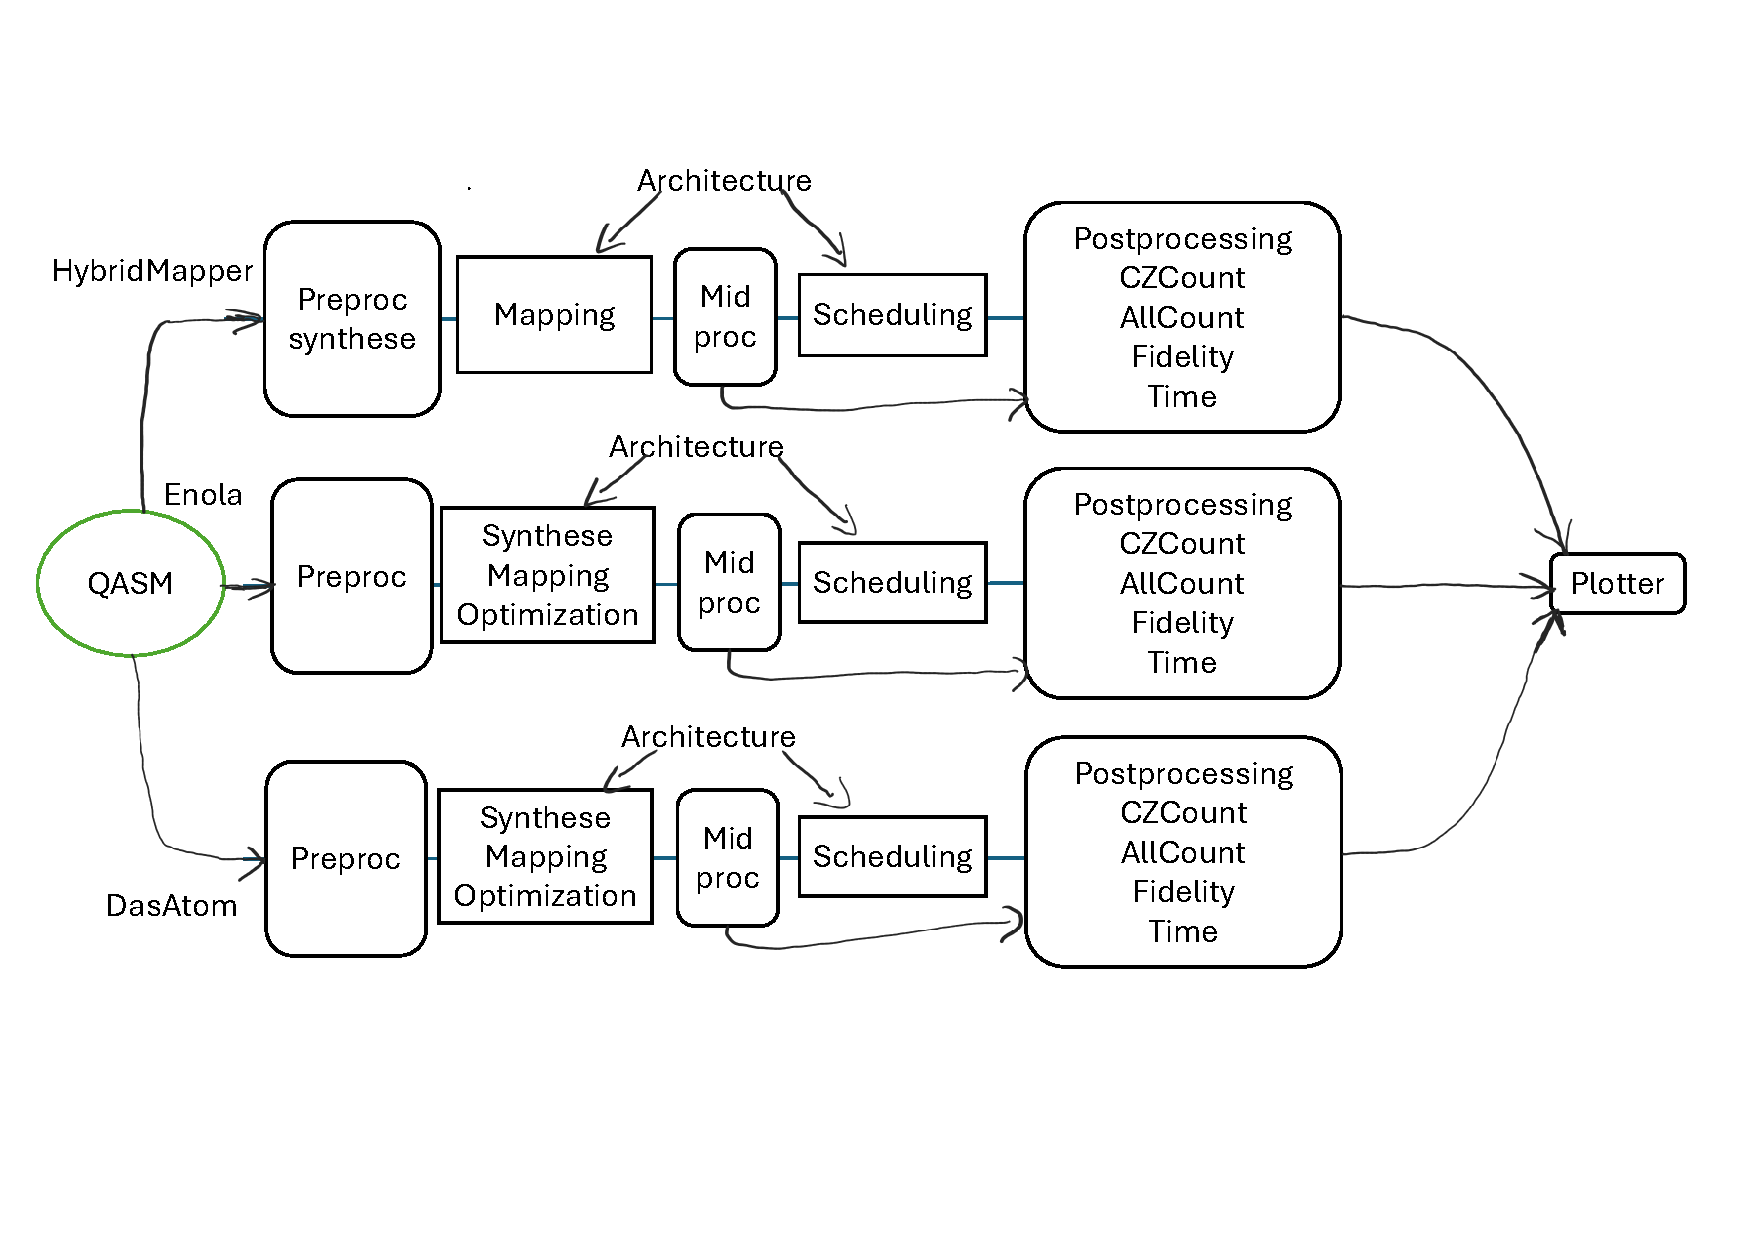
\includegraphics[width=1.0\textwidth]{figures/schema.pdf}
    \caption{Workflow of benchmarking script}
    \label{fig:overview}
\end{figure}
Since all considered compilers are not actually a compiler in the full sense, but rather tool chains with different tools
a multitude non-trivial architecture adaptations, pre-processing, mid-processing and post-processing steps were required. 

\section{First Evaluation}
Here are main architecture parameters for first evaluation \ref{tab:architecture_first}. 
Then they were adapted as similar as possible to pass into each compiler's own input form, as a result, small inaccuracies may occur.
\begin{table}[htpb]
  \caption[Architecture First Run]{Architecture parameters for first run}\label{tab:architecture_first}
  \centering
  \begin{tabular}{l l l l}
    \toprule
      Parameter & Value \\
    \midrule
      Interaction Radius & 2 \\
      Rydberg Blockade & 2 \\
      Two Qubit Time & 0.36 \\
      One Qubit Time & 0.36 \\
      Two Qubit Fidelity & 0.9999 \\
      One Qubit Fidelity & 0.9999 \\
      Coherence Time $\mu$s & 1500000 \\
      AOD Activate Time $\mu$s & 20 \\
      Move Fidelity  & 0.9999 \\
      Move Speed $\mu$m/$\mu$s & 0.55 \\
      SLM AOD separation & 2\\
    \bottomrule
  \end{tabular}
\end{table}

The following results were obtained \ref{fig:AllGateCountArch1},
\ref{fig:CZGateCountArch1}, \ref{fig:FidelityArch1}. 
Nevertheless, due to very long compilation time Enola was tested separately in \ac{QFT}30 \ref{tab:EnolaDasAtomQFT30}.
\begin{figure}[htbp]
  \centering
    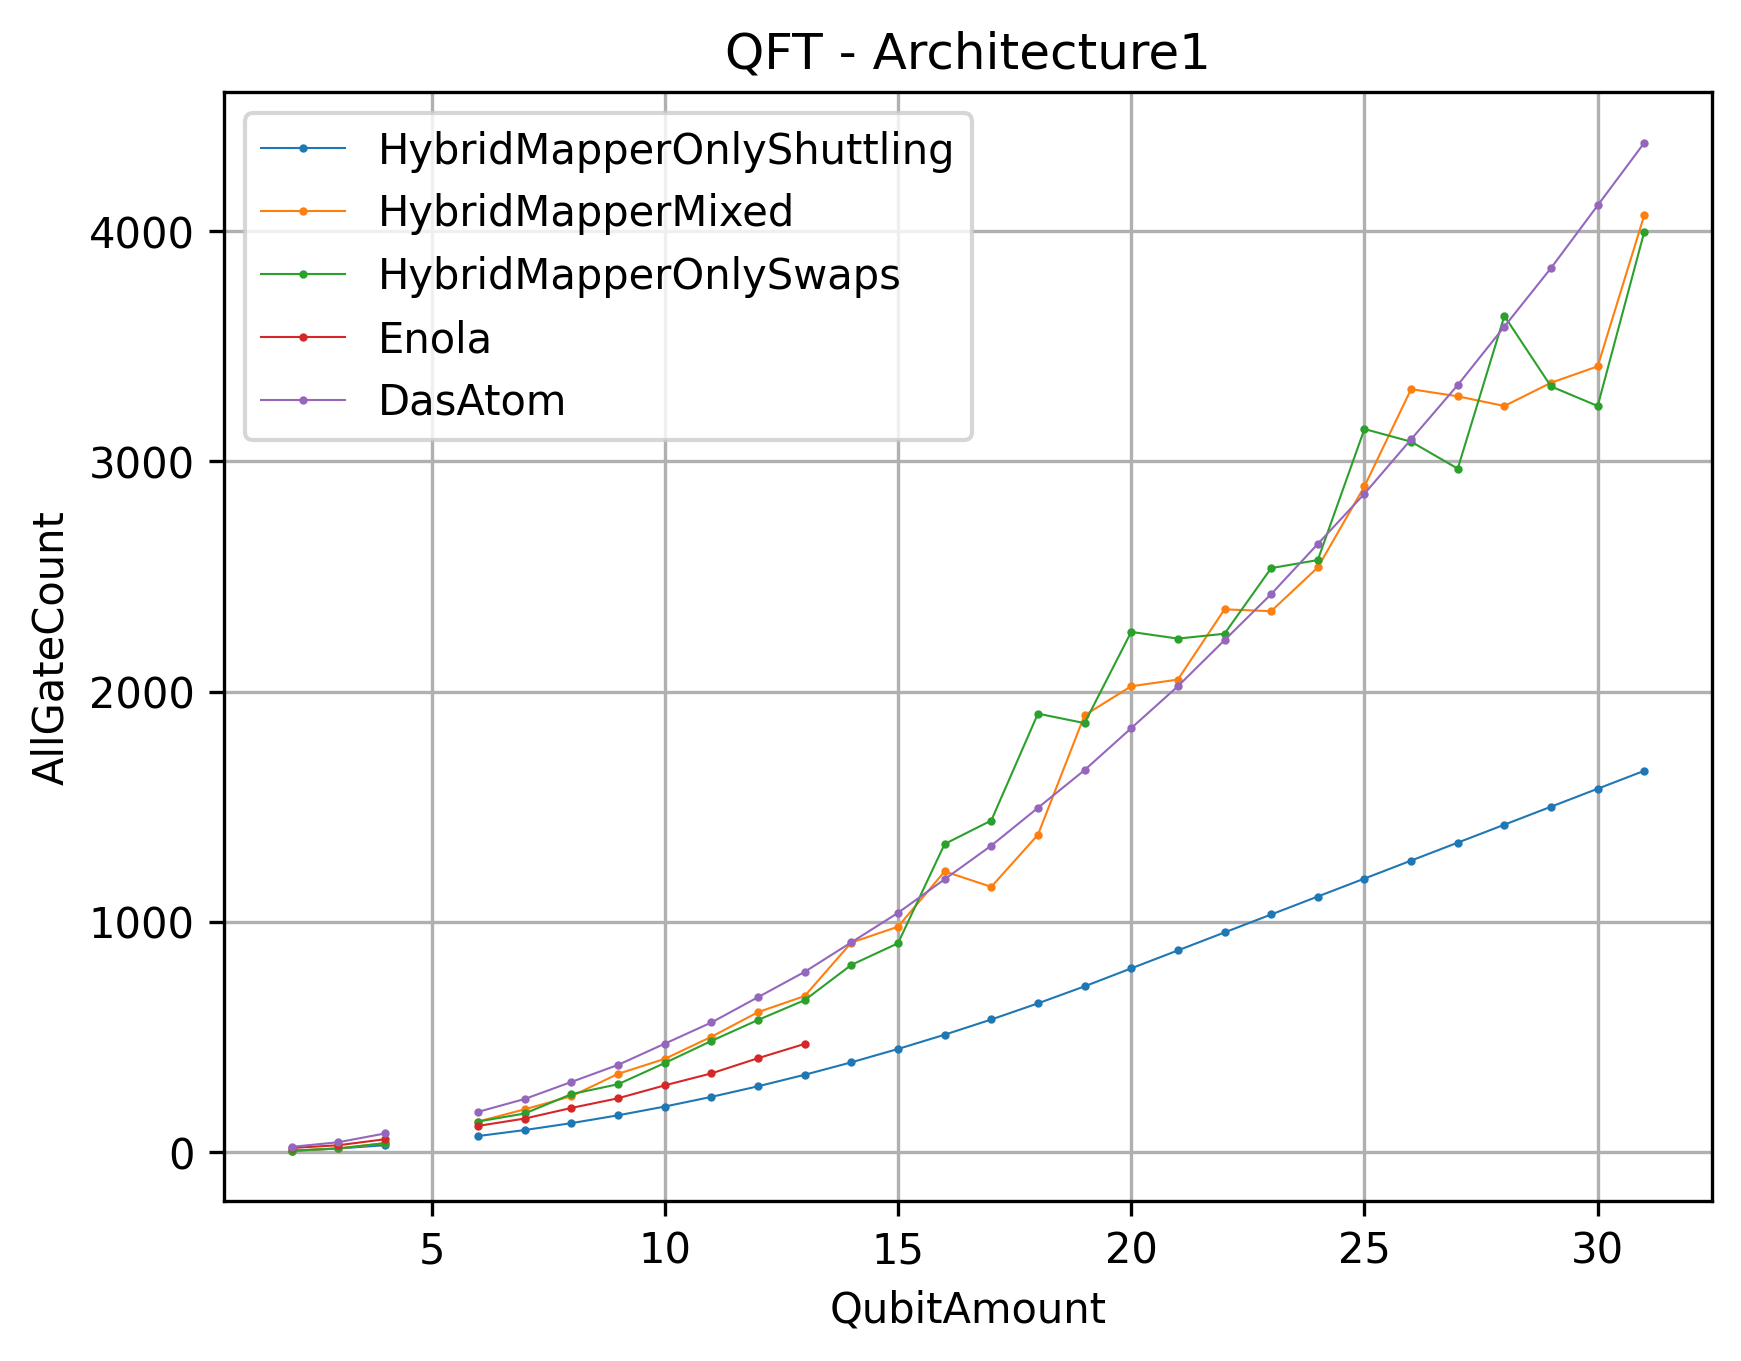
\includegraphics[width=0.7\textwidth]{figures/AllGateCountArch1.png}
    \caption[All Gate Number of first Architecture]{Number of All Gates in compiled Circuit in first architecture}
    \label{fig:AllGateCountArch1}
\end{figure}
\begin{figure}[htbp]
  \centering
    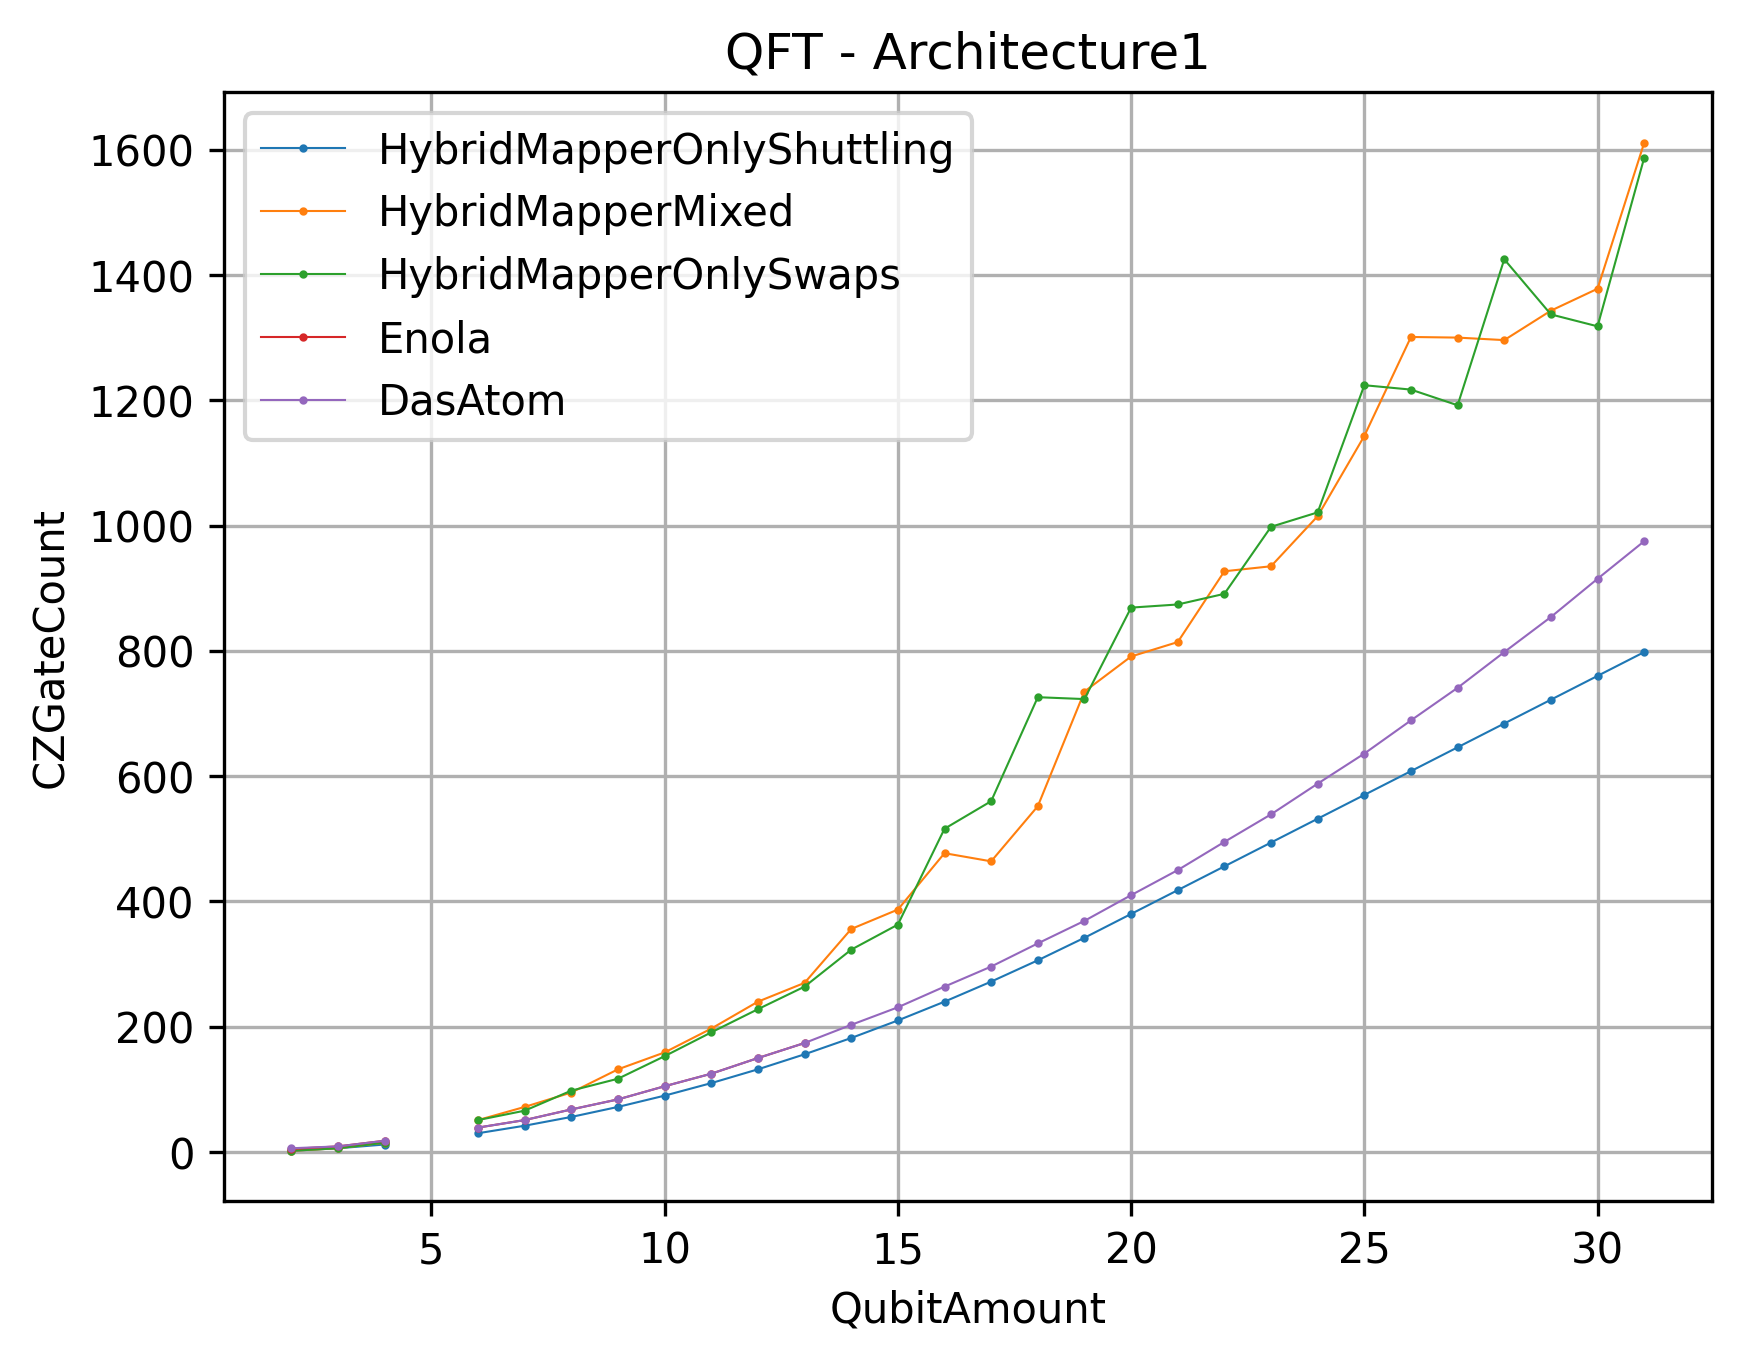
\includegraphics[width=0.7\textwidth]{figures/CZGateCountArch1.png}
    \caption[CZ Gate Number for first Architecture]{Number of CZ Gates in compiled Circuit in first architecture}
    \label{fig:CZGateCountArch1}
\end{figure}
\begin{figure}[htbp]
  \centering
    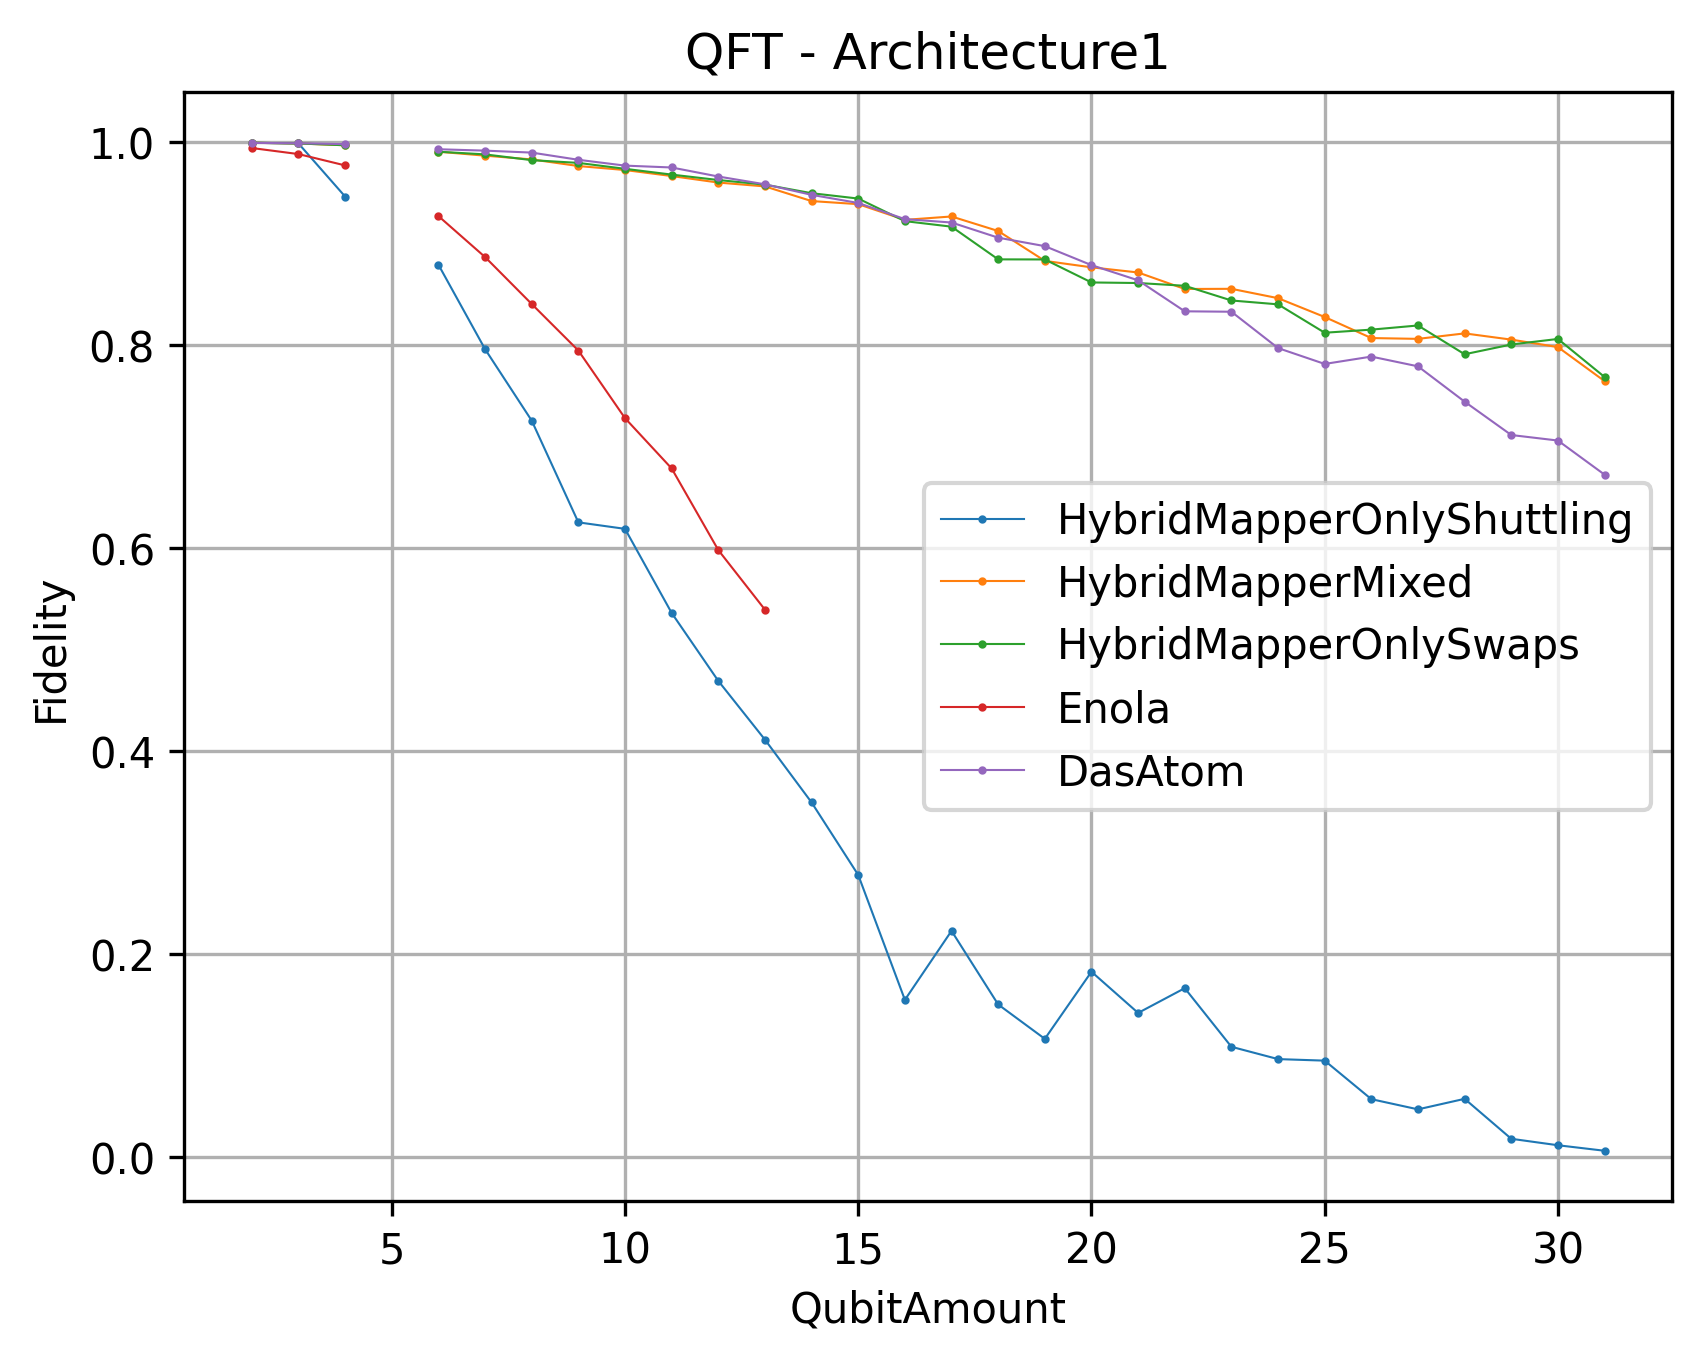
\includegraphics[width=0.8\textwidth]{figures/FidelityArch1.png}
    \caption[Fidelity in first Architecture]{Fidelity in first Architecture}
    \label{fig:FidelityArch1}
\end{figure}
\begin{table}[htpb]
  \caption[Enola DasAtom First Run QFT30]{Enola DasAtom First Run QFT30}\label{tab:EnolaDasAtomQFT30}
  \centering
  \begin{tabular}{l l l l}
    \toprule
      Output & Enola QFT30 & DasAtom QFT30 \\
    \midrule
      Fidelity Overall & 0.0008991 & 0.7060\\
      Fid. Movement & 0.69376 & 0.9934373\\
      Fid. Coherence & 0.00154 & 0.81603\\
      Gate Count & 2370 & 4111\\
      CZ Gates & 915 & 915\\
      Fid. 1Q & 1 & 1\\
      Compile Time s & 14251 & 2.5\\
    \bottomrule
  \end{tabular}
\end{table}

\subsection{Result Interpretation}
Firstly, one can observe \ref{fig:AllGateCountArch1} that number of used gates by \ac{HM} with Shuttling-based strategy is the lowest, 
when other tools require significantly more gates. It is a case, because \ac{HM} in shuttling mode only make moves and does not change a circuit,
when other actively change input circuit and \ac{HM} in SWAP-based mode uses a CZ with Hadamard gates to solve a coupling problem \parencite{schmid2023hybridcircuitmappingleveraging,Emil_Khusainov_Bachelor_GIT}.

Secondly, one can see in \ref{fig:AllGateCountArch1}, in \ref{tab:EnolaDasAtomQFT30}, 
and in \ref{fig:CZGateCountArch1} that Enola uses considerable fewer gates one-qubit Gates than DasAtom. 
But when one sees an output of compilation, 
then a fidelity of one-qubit gates is equal to 1.0 
since both Enola and DasAtom do not consider impact of one-qubit gates onto fidelity.
Taking into account that DasAtom states 415x times more fidelity than Enola, 
but in same time uses more and not consider one-qubit gates. This may result in a comparison that favors one toolchain over the others.
For example, for fidelity of one-qubit gates equal 0.9999: \[0.9999^{4111 - 2370} \approx 0.84\]
What would bring a valuable impact on overall fidelity.

Thirdly consider \ref{fig:FidelityArch1} and \ref{tab:EnolaDasAtomQFT30}, \ac{QFT} is not a very large circuit, 
and parameters for physical \ac{AOD} and \ac{SLM} grid were considerable similar.
It is worth investigating the reasons behind this difference in move fidelity and coherence fidelity between Enola and DasAtom.
Recall that DasAtom states a significant outperform of Enola and according to results of first run fidelity difference were around 700x times, 
what is similar in inaccuracy with 414x times \parencite{huang2025dasatomdivideandshuttleatomapproach}.

Fourthly, it is notable that optimization of DasAtom achieve the same fidelity as Swap Based \ac{HM}, 
when DasAtom uses only shuttling and \ac{HM} with shuttling is substantially worse.

\section{Justification and correction of differences}
To find out the reason for such a strong difference a source codes of corresponding gits 
of Enola \parencite{Tan_2025_Enola} and DasAtom \parencite{huang2025dasatomdivideandshuttleatomapproach} were investigated \parencite{Emil_Khusainov_Bachelor_GIT}.

\subsection{Single Qubit Fidelity}
Recall that DasAtom and Enola does not consider one-qubit gates into fidelity calculation.
Nevertheless, Enola introduces one-qubit fidelity calculation in its paper, 
however, in the actual source code this value is hardcoded as 1.0 and remains unused \parencite{Emil_Khusainov_Bachelor_GIT,Tan_2025_Enola}.
Therefore, such functionality to both compilers was added according to well-known formula: \[fidelity_{\mathrm{1Q}}^{N_{\mathrm{1Q}}}\]

\subsection{Investigating Different Coherence Fidelity}
In Enola according to source codes, and it's paper following formula for fidelity coherence is used:
\[\prod_{q \in Q} \left(1 - \frac{t_q}{T_2} \right)\]
It is a first order Taylor expansion and enough precise, but better to use an exponential variation which is used in DasAtom:
\[e^{-t / T_2}\]

After applying modifications, Enola calculates coherence fidelity with: \[\prod_{q \in Q} \left(e^{-t_q /  T_2} \right)\]

\subsection{Investigating Different Move Idle Time for Coherence}
During improving of Enola behavior, was noticed, that an idle time t is significantly different for Enola compared to the other two.
The search revealed the reason for this difference; DasAtom and \ac{HM} use simple linear formula to calculate time for movement: \[distance/speed\]
Nevertheless, Enola used an approach described by Dolev Bluvstein to calculate move time:
\[200 \sqrt{\frac{distance}{110}}\]
This approach does not consider different possible architectures and therefore speed and distances. 
It was created to show a non-linear dependency between time and distance e.g. due to acceleration and slowdown.
But when distance is not equal to 110 then a difference between resulting times of approaches grows drastically.
Hence, for honest testing Enola will use also linear approach.

\subsection{Investigating Different Move Distances}
The following issues were noticed during repair of move time calculation \parencite{Emil_Khusainov_Bachelor_GIT}. 
Move distance was very different between DasAtom and Enola. 
For example, when average movement on DasAtom was 11 $\mu$m, on Enola it was more than 200 $\mu$m. 
That was strange and needed further investigation.

As a result a significant source code error was found. 
The Enola compiler does not consider architecture parameters on mapping and routing steps, only on scheduling.
Therefore, from the outside it looked like there was some kind of reaction to the architecture changes.
But in mapping and routing step the architecture parameters were defined as global variables, 
when a Set function does not consider those as global, but creates local variables with same name.
This mistake was fixed and changes could be evaluated again.

\section{Second Evaluation}
Here are slightly revised new architecture parameters based on increased experience working with these toolchains.
Changed was a \ac{AOD} activate time from 20 $\mu$s to 0.55 $\mu$s due to the diverse utilizations of this parameter,
and therefore different impact on similar \ac{AOD} sequences.
Moreover, fidelity of two-qubit gates were downgraded from 0.9999 to 0.9996 
due to added consideration of one-qubit gates with fidelity 0.9999,
and obvious that two-qubit gates should have then lower fidelity.
\begin{table}[htpb]
  \caption[Architecture Second Run]{Architecture parameters for second run}\label{tab:architecture_second}
  \centering
  \begin{tabular}{l l l l}
    \toprule
      Parameter & Value \\
    \midrule
      Interaction Radius & 2 \\
      Rydberg Blockade & 2 \\
      Two Qubit Time & 0.36 \\
      One Qubit Time & 0.36 \\
      Two Qubit Fidelity & 0.9996 \\
      One Qubit Fidelity & 0.9999 \\
      Coherence Time $\mu$s & 1500000 \\
      AOD Activate Time $\mu$s & 0.55 \\
      Move Fidelity  & 0.9999 \\
      Move Speed $\mu$m/$\mu$s & 0.55 \\
      SLM AOD separation & 2\\
    \bottomrule
  \end{tabular}
\end{table}

The following results were obtained \ref{fig:AllGateCountArch2},
\ref{fig:CZGateCountArch2}, \ref{fig:FidelityArch2}.
\begin{figure}[htbp]
  \centering
    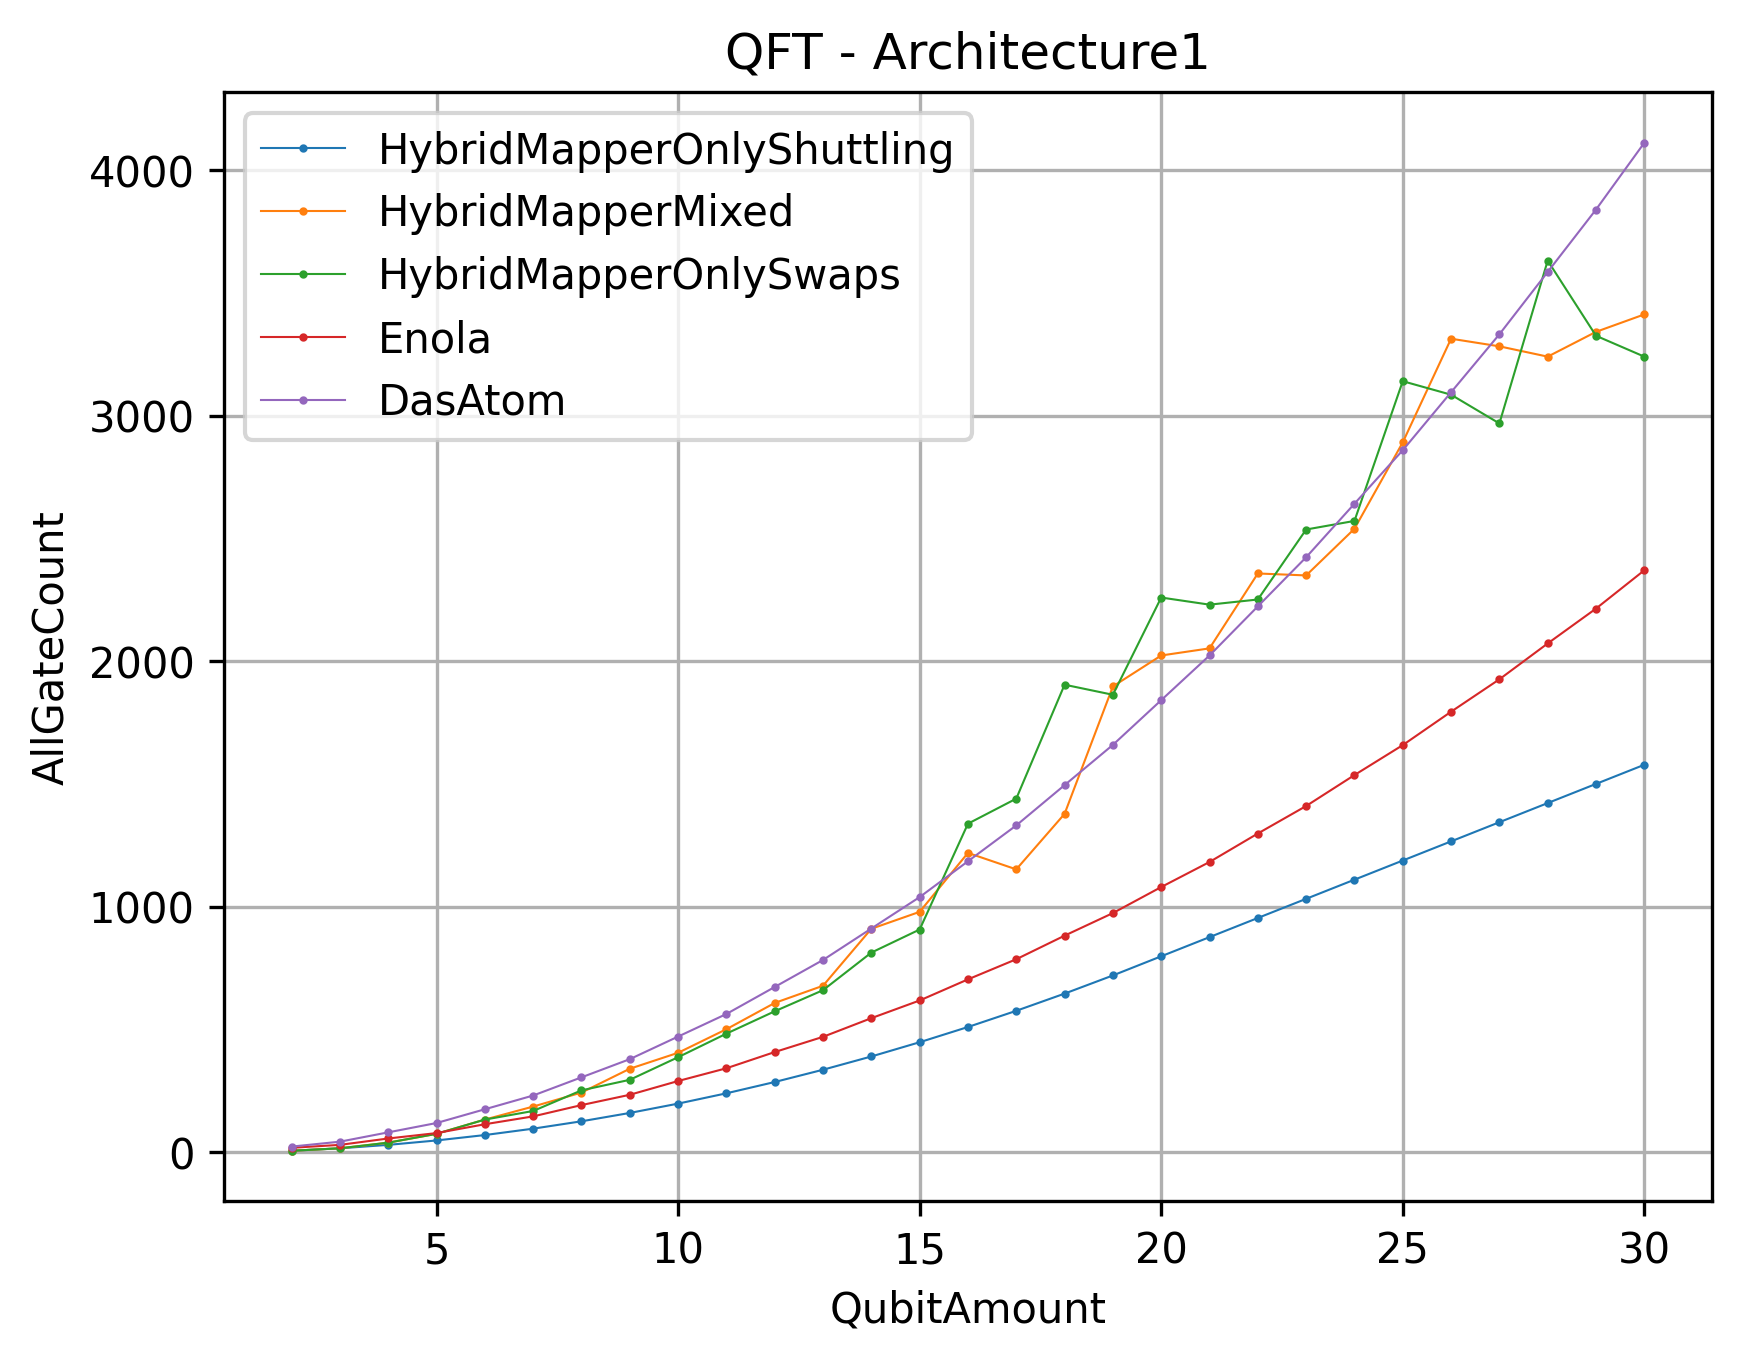
\includegraphics[width=0.7\textwidth]{figures/AllGateCountArch2.png}
    \caption[All Gate Number of second Architecture]{Number of All Gates in compiled Circuit in second architecture}
    \label{fig:AllGateCountArch2}
\end{figure}
\begin{figure}[htbp]
  \centering
    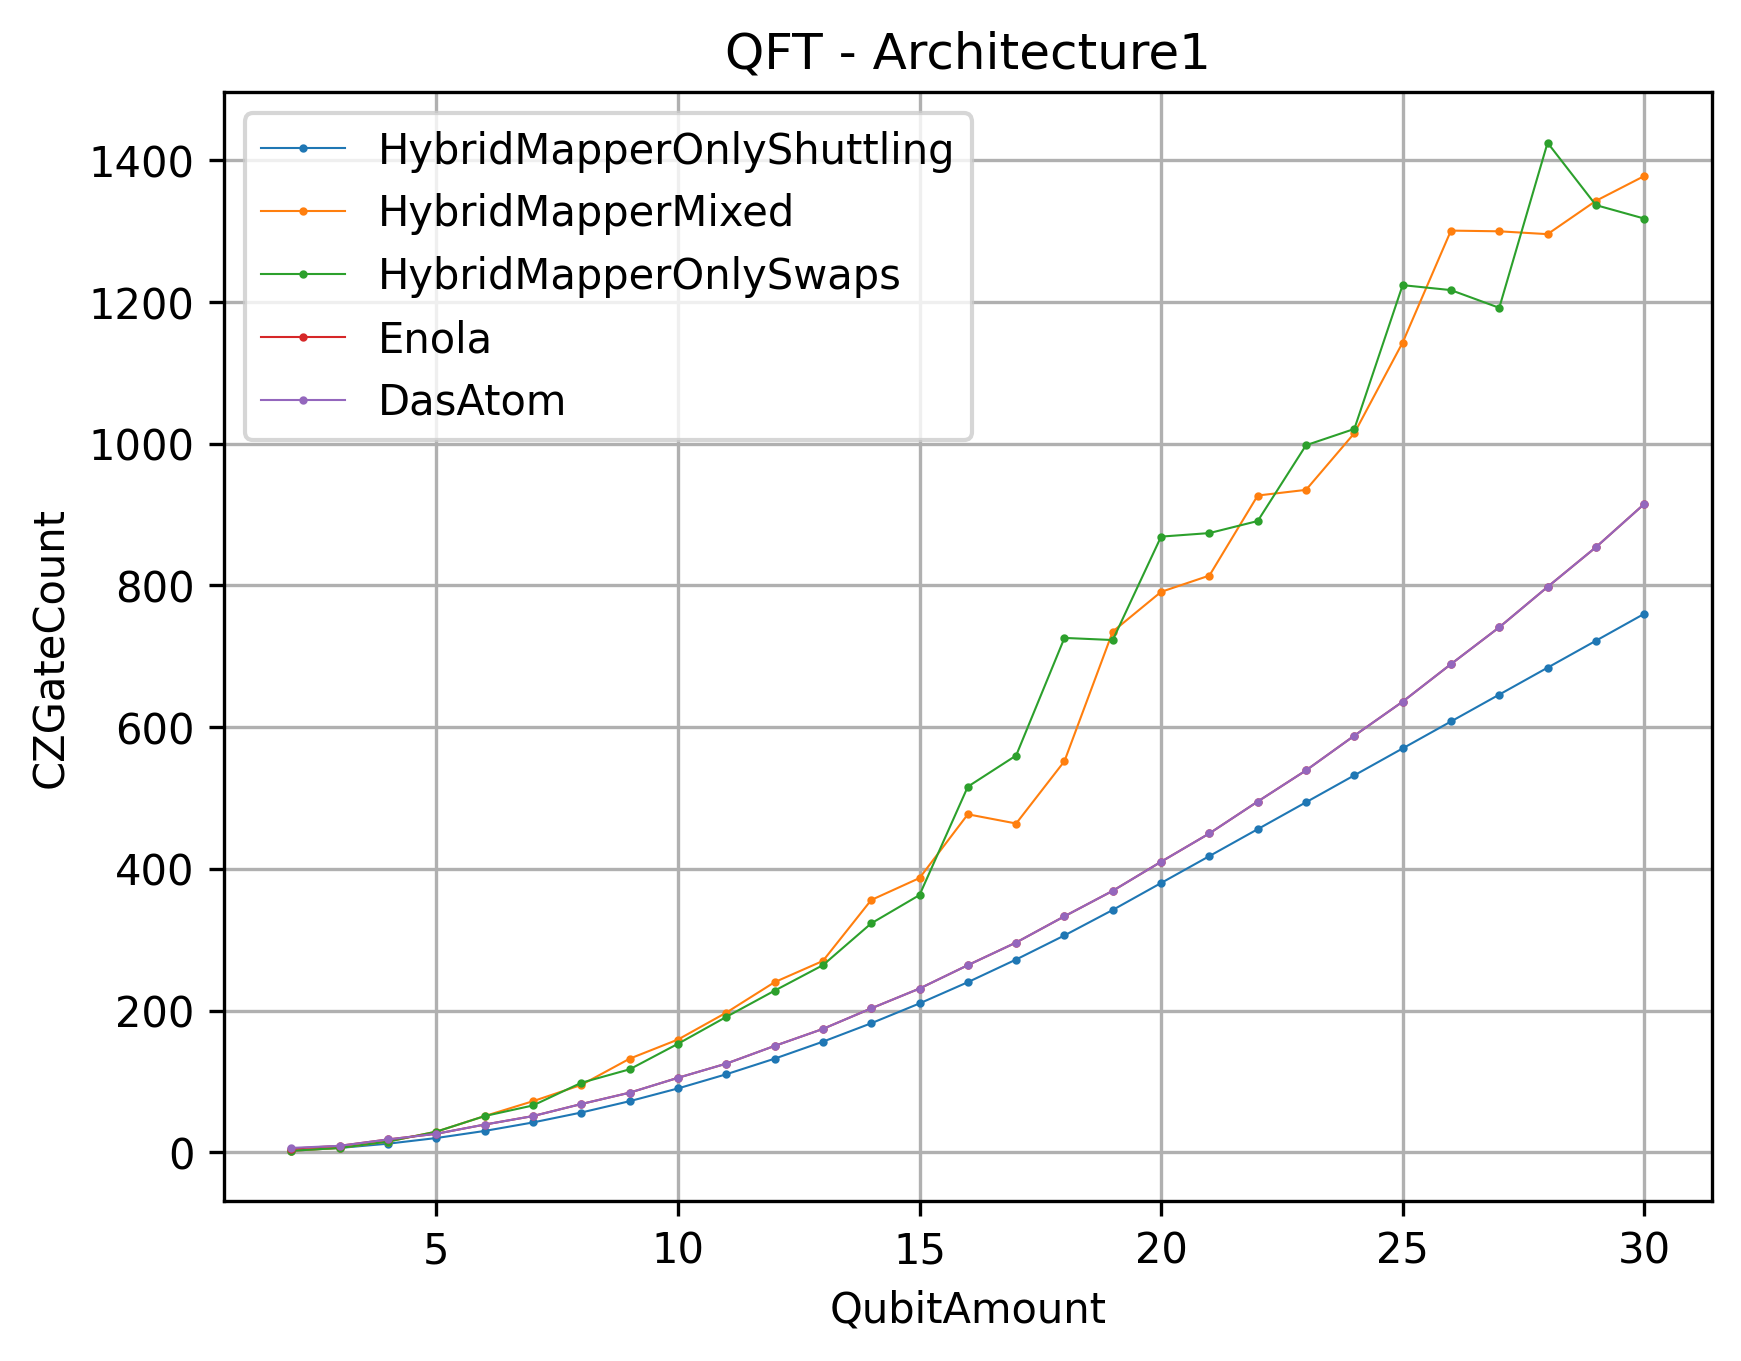
\includegraphics[width=0.7\textwidth]{figures/CZGateCountArch2.png}
    \caption[CZ Gate Number for first Architecture]{Number of CZ Gates in compiled Circuit in second architecture}
    \label{fig:CZGateCountArch2}
\end{figure}
\begin{figure}[htbp]
  \centering
    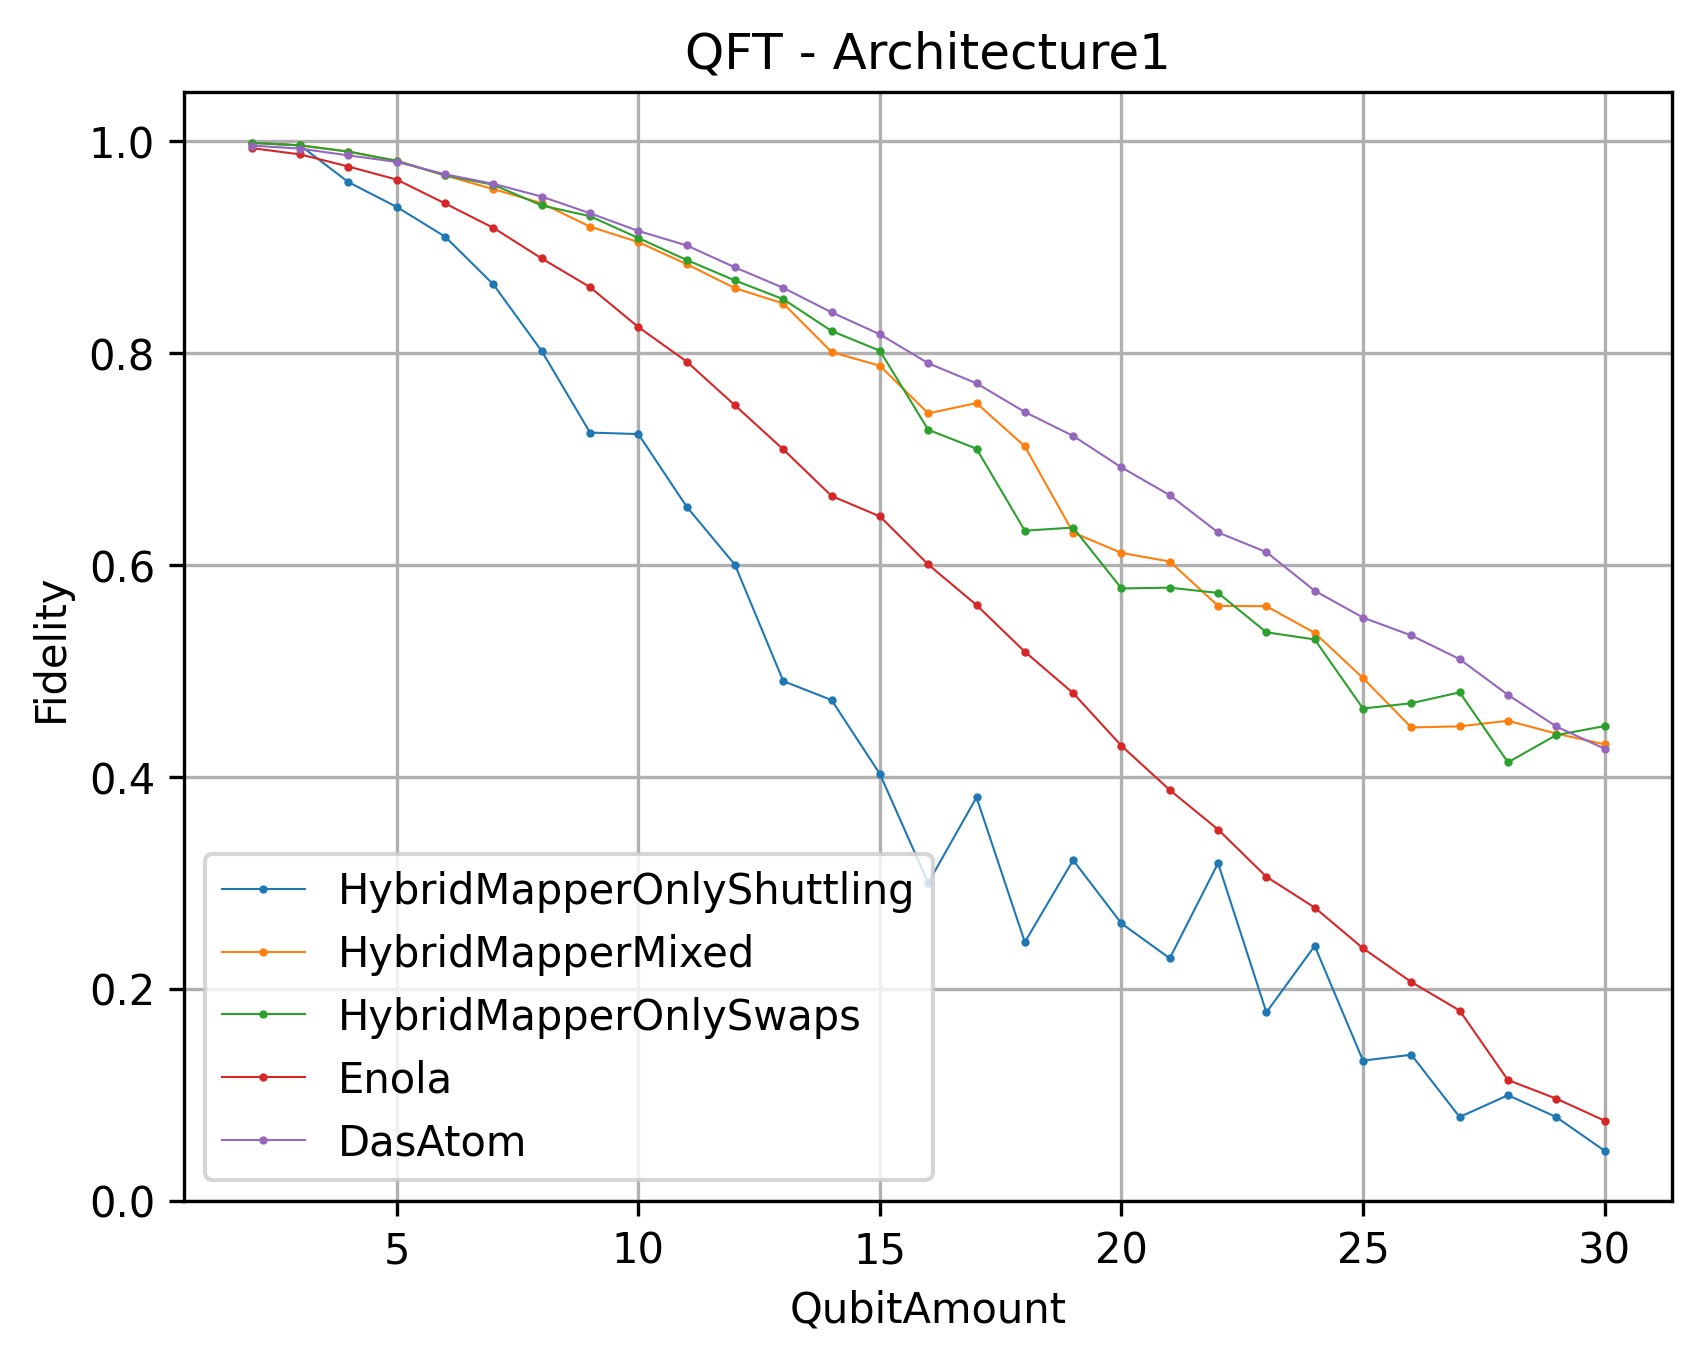
\includegraphics[width=0.8\textwidth]{figures/FidelityArch2.png}
    \caption[Fidelity in second Architecture]{Fidelity in second Architecture}
    \label{fig:FidelityArch2}
\end{figure}

\subsection{Result Interpretation}
Firstly, one can observe in \ref{fig:FidelityArch2} that difference between DasAtom and Enola for \ac{QFT}30 is only about 5.5 times higher,
and an exponentially increasing gap is not observed.
Moreover, Enola consider a lot more fidelity affecting factors that were not considered here and not investigated, 
but have a considerable effect on fidelity. 
Therefore, it is likely that, under fair consideration of all co-factors the result difference will be slightly less than 5.5 times.

Secondly, \ref{fig:FidelityArch2} confirms that Enola is a bit better than shuttling based \ac{HM}, due to missing optimization step in \ac{HM}
and DasAtom could achieve a SWAP level fidelity by using only shuttling and sometimes outperform \ac{HM} with enabled SWAP.
Nevertheless, one should not forget that an input QFT is a optimized already by input and perhaps on random circuit the results will be different.

% !TeX root = ../main.tex
% Add the above to each chapter to make compiling the PDF easier in some editors.

\chapter{Future Work}\label{chapter:futurework}
Taken together, much work remains to be done. 
Firstly, such as adding new compiler toolchains for comparison 
and developing a universal framework to manage input, 
and output results, and moreover to fair calculate and interpret statistics.
Or something of greater depth, 
such as consideration of all possible parameters that take place for example in Enola but do not in other,
and due to not very big impact on calculations, frequently it is not being considered.
Moreover, different circuits could be used, with different level of start optimizations to see actually performance of a tool chain.

Very valuable scientific contribution would be to test compiler tool chain on a real hardware.
This would allow for fairer comparisons and a more accurate interpretation towards a potential unified framework.
But is it a bit difficult due to the lack of public available \ac{NAQC}. 
Particular ones of them do not expose in API a possibility to shuttle qubit in runtime, such as Aquila from Amazon.
Other, work on a very low level of analog pulses, such as Pasqal Pulser, what creates more constraints onto testing of High-level toolchains.
% !TeX root = ../main.tex
% Add the above to each chapter to make compiling the PDF easier in some editors.

\chapter{Conclusion}\label{chapter:conclusion}
\ac{NAQC} represent a new hardware architecture with exclusive combination of capability and constraints.
This architecture has significant perspectives in world of quantum computations. 
Nevertheless, to subjugate all the power of it a good software solution must be produced.

This work was focused on benchmarking of existing compilation toolchains 
and the most important thing is an honest comparison. What was fullified in this paper.

Firstly, a test setup was created, to bring all tool chains into similar conditions, and first testing was performed.

Secondly, results were interpreted, and suspicious things were investigates and repaired.

Thirdly, the new testing was performed, that has shown a worthy results 
such as finding that difference is actually not a 400x times and exponential grow as DasAtom \parencite{huang2025dasatomdivideandshuttleatomapproach} states, 
but either 5.5x times between Enola and DasAtom \parencite{Emil_Khusainov_Bachelor_GIT}. 

% TODO: add more chapters here

\appendix{}

\microtypesetup{protrusion=false}

\addchap{Abbreviations}
\begin{acronym}
	\itemsep-.25\baselineskip
	\acro{TUM}[TUM]{Technical University of Munich}
	\acro{DPQA}[DPQA]{Dynamically Field-Programmable Qubit Arrays}
	\acro{NAQC}[NAQC]{Neutral Atom Quantum Computer}
	\acro{QC}[QC]{Quantum Computer}
	\acro{NISQ}[NISQ]{Noisy Intermediate Scale Quantum Computing Era}
	\acro{FTQC}[FTQC]{Fault-Tolerant Quantum Computing Era}
	\acro{SLM}[SLM]{Spatial Light Modulator}
	\acro{AOD}[AOD]{Acousto-Optic Deflector}
	\acro{MQT}[MQT]{Munich Quantum Valey}
	\acro{UCLA-VAST}[UCLA-VAST]{UCLA-VAST Lab}
	\acro{QFT}[QFT]{Quantum Fourier transform}
	\acro{DAC}[DAC]{Divide-and-conquer}
	\acro{HM}[HM]{HybridMapper}
	% TODO: add acronyms
\end{acronym}

\listoffigures{}
\listoftables{}
\microtypesetup{protrusion=true}
\printbibliography{}

\end{document}
